\documentclass[]{article}

% Packages
\usepackage{amsmath} % math stuff
%\usepackage[dvipsnames]{xcolor}  % for coloring
\usepackage{tensor}  % tensors, but also for stuff like superscript on the left
\usepackage{enumitem} % for enumerating alphabetically
\usepackage{tabto}		% for tabbing to a certain length
\usepackage{scrextend} % for local margins
\usepackage{titling}	% for subtitle custom command
\usepackage[svgnames, table]{xcolor} % avoid the option clash for hyperref command  + TABLE REP
\usepackage[colorlinks=true, linkcolor=Blue, urlcolor=Blue]{hyperref} % for hyperref command 
\usepackage{pgfplots} % plots
\usepackage{circuitikz} % circuit plots
\usetikzlibrary{positioning} % positioning in circuit plots
\usetikzlibrary{backgrounds, shapes} % shapes for multiplexer+
%%\usepackage{outlines} % convienent itemizing

%for flowchart:
\usepackage{amsmath}
\usepackage{amssymb}
\usepackage{graphicx}
\usepackage{siunitx}
\usepackage{tikz}
\usetikzlibrary{patterns}
\usepackage{caption}
\usetikzlibrary{arrows}
\usepackage{color}
\usepackage{pgfplots}
\usepackage{listings}
\usepackage[utf8]{inputenc}
\usetikzlibrary{shapes.geometric}
\usepackage{tikz-cd}
\usetikzlibrary{positioning}
\tikzset{
	shift left/.style ={commutative diagrams/shift left={#1}},
	shift right/.style={commutative diagrams/shift right={#1}}
}


%tables for list representation
\usepackage{arydshln, collcell}
\newcolumntype{C}{>{\collectcell\mathsf}c<{\endcollectcell}}


%Repeat command
\usepackage{expl3}
\ExplSyntaxOn
\cs_new_eq:NN \Repeat \prg_replicate:nn
\ExplSyntaxOff

% Algorithms
\usepackage{algorithm}
\usepackage{algorithmicx}
\usepackage[noend]{algpseudocode}
\newcommand{\Get}{\State \textbf{get}~}
\newcommand{\Set}{\State \textbf{set}~}
\newcommand{\Print}{\State \textbf{print}~}
\newcommand{\Getx}[1]{\Statex \algindent{#1} \textbf{get}~}		% x denotes non-numbered lines
\newcommand{\Setx}[1]{\Statex \algindent{#1} \textbf{set}~}	% enter the number of lines to indent
\newcommand{\Printx}[1]{\Statex \algindent{#1} \textbf{print}~}
\newcommand{\Stop}{\State \textbf{stop}~}
\newcommand{\algindent}[1]{\Repeat{#1}{\hskip\algorithmicindent}}
\algdef{SE}[DOWHILE]{Do}{doWhile}{\algorithmicdo}[1]{\algorithmicwhile\ (#1)}


% stop indentation
\setlength{\parindent}{0pt}

% custom subtitle command
\newcommand{\subtitle}[1]{
	\posttitle{
		\par\end{center}
	\begin{center}\large#1\end{center}
	\vskip0.5em}
}


% Fixes weird backwards quote thing
\usepackage [english]{babel}
\usepackage [autostyle, english = american]{csquotes}
\MakeOuterQuote{"}

% fix upside down exclaimation points for less thans or greater thans
\usepackage[T1]{fontenc}


% Title
\title{CS 201 Notes}
\subtitle{Introduction to Computer Science}
\author{Jaeden Bardati}
\date{\textit{Last modified \today}}

\setcounter{section}{-1}	% 0-indexes the section

\begin{document}

\maketitle
\bigbreak

% Course Video 0
\section{Course Overview\\ {\large \normalfont September 10, 2021}}
\bigbreak

\subsection{What is Computer Science?}
\bigbreak

Computer science is the study of \textbf{algorithms}.\\\\
An \textbf{algorithm} is an effective method for solving a problem, expressed as a finite sequence of steps.\\\\
The development of algorithms works in this recurring order:
\begin{itemize}
	\item \textbf{Design}
	\item \textbf{Analysis}
	\item \textbf{Implement}
	\item \textbf{Experiment}\smallskip
\end{itemize}

\noindent In the \textbf{design} phase, we design an algorithm using pseudo-code. In the \textbf{analysis} phase, we need to analyze the correctness and the efficiency. That is to say, we make sure that our algorithm will work and completes in a reasonable amount of time. During the \textbf{implementation}, the algorithm is written in code on a computer. Finally, the algorithm is run and debugged in the \textbf{experiment} phase. This process repeats.


\section{Introduction to Algorithms}
\bigbreak

% Course Video 1
\subsection{Design\\ {\normalfont September 11, 2021}}
\bigbreak

An algorithm is a step by step procedure to solve a problem. For example, 
\begin{itemize}
	\item Step 1: Do something
	\item Step 2: Do something
	\item ...
	\item Step n: Do something\smallskip
\end{itemize}

\noindent There are three basic types of steps. Note that there is a fourth (recursion), but it is not covered in this course. 
\subsubsection{Sequential Steps}
\bigbreak
	\textbf{Do a single task}.\\\\
	\textit{For example:} Let $x$ be a variable. A sequential step could be to add 1 to $x$.
\subsubsection{Conditional Steps}
\bigbreak
	\textbf{Ask a question} that supports only \textbf{logic answers} (true or false answer). \\\\
	\textit{For example:} Let $x$ be a variable. A conditional step could be to ask if $x > 0$. If so, add 1 to $x$; otherwise, subtract 1 from $x$.
\subsubsection{Iterative Steps (loops)}
\bigbreak
	\textbf{Repeat a task} until a certain condition is satisfied. This step links the sequential step to the conditional steps.\\\\
	\textit{For example:} If you have a recipe that you need to add water until its dry. An iterative step would be one where you add $\frac{1}{2}$ cup to mixture while mixture is dry.


% Course Video 2 and 3
\subsection{Case Study: Addition Algorithm\\ {\normalfont September 11, 2021}}
\bigbreak

Let's say we want to add 472 to 593. We would to it like so:\\\\
\begin{tabular}{cccc}
	& \tiny 1 & \tiny & \tiny \\
	& 4 & 7 & 2 \\
	+ & 5  & 9 & 3 \\
	\hline
	1 & 0 & 6 & 5 \\
\end{tabular}
\medbreak
\noindent If you know how to add these numbers, you know how to do it for any numbers. Why? Because we used a sequence of steps to solve it: We used an algorithm. What is this algorithm?\\

\noindent We know that we can break down the work for each of the digits. It is an iterative statement for each digit. What is the work we need to do at each iteration?\\

\noindent First, we add the digits plus the carry in (starts at 0). This is a \textbf{sequential step}. Then, we ask if it is greater than 9. If so, we set the resulting digit as the addition subtracted by 10 and set the carry out (which is te carry in for the next step) to 1; otherwise, we simply set the resulting digit as the addition and set the carry out to be 0. This is a \textbf{conditional step}. Then we repeat this process until we have no more digits to add. This is an \textbf{iterative step}.\\

\noindent Now, we need to conceptualize this. Let's let $m \geq 1$ be the number of digits. Let us define $a_i$ (first number digits), $b_i$ (second number digits) and $c_i$ (resulting number digits) as follows:

\begin{tabular}{ccccc}
	& \tiny & \tiny & \tiny & \tiny \\
	& $a_{m-1}$ & ... & $a_{1}$ & $a_{0}$ \\
	+ & $b_{m-1}$ & ... & $b_{1}$ & $b_{0}$ \\
	\hline
	$c_{m}$ & $c_{m-1}$ & ... & $c_{1}$ & $c_{0}$ \\\smallskip
\end{tabular}

\noindent Let's write the steps of our algorithm:

\begin{algorithm}
	\caption{\\Addition Algorithm}
	\begin{algorithmic}[1]
		\Get $m$ (provided by user)
		\Get $a_{m-1}$, ...  $a_{1}$, $a_{0}$ and $b_{m-1}$, ...  $b_{1}$, $b_{0}$ (provided by user)
		\Set $i = 0$ (digit index) and carry = 0
		\While{($i \leq m - 1$)}
			\Set $c_i = a_i + b_i$ + carry
			\If{($c_i \geq 10$)}
				\Set $c_i = c_i - 10$
				\Set carry = 1
			\Else
				\Set carry = 0
			\EndIf
			\Set $i = i + 1$
		\EndWhile
		\Set $c_m$ = carry
		\Print $c_{m-1}$, ...  $c_{1}$, $c_{0}$
		\Stop
	\end{algorithmic}
\end{algorithm}

\noindent This can be programmed now using a programming language.\\

\noindent If you want to test your algorithm, you can perform a \textbf{trace}. A trace is when you go through the algorithm yourself step by step for a test case.


% Course Video 4, 5, 6 and 7
\subsection{Pseudocode\\ {\normalfont September 11, 2021}}
\bigbreak

Pseudocode is:

\begin{itemize}
	\item Simplified
	\item A tradeoff between natural and programming languages
	\item Not unique\smallskip
\end{itemize}

\noindent We will now look into the types of statements and the syntax we will use.

\subsubsection{Sequential statements}
\bigbreak
\begin{itemize}
	\item \textbf{Input}: Get "variable". E.g. Get $m$, Get radius
	\item \textbf{Computation}: Set variable = expression. E.g. Set area = $\pi \times$ radius$^2$
	\item \textbf{Output}: Print "variable". E.g. Print area.\smallskip
\end{itemize}

\begin{algorithm}
	\caption{\\Calculates the average of three numbers.}
	\begin{algorithmic}[1]
		\Get $x, y, z$
		\Set average = $\frac{x + y + z}{3}$
		\Print average
		\Stop
	\end{algorithmic}
\end{algorithm}

\subsubsection{Conditional statements}
\bigbreak
\begin{itemize}
	\item If (condition) Then\\
				\tabto{0.5cm}operation T$_1$\\
				\tabto{0.5cm}operation T$_2$\\ 
				\tabto{0.5cm}...\\
				\tabto{0.5cm}operation T$_\mathrm{m}$\\
			Else\\
				\tabto{0.5cm}operation F$_1$\\
				\tabto{0.5cm}operation F$_2$\\ 
				\tabto{0.5cm}...\\
				\tabto{0.5cm}operation F$_\mathrm{n}$\smallskip
\end{itemize}

\begin{algorithm}
	\caption{\\Print average of three number if the first number is larger than 0, otherwise print an error message.}
	\begin{algorithmic}[1]
		\Get $x, y, z$
		\If{($x \geq 0$)}
			\Set average = $\frac{x + y + z}{3}$
			\Print average
		\Else	
			\Print "Bad Data"
		\EndIf
		\Stop
	\end{algorithmic}
\end{algorithm}

\noindent When a conditional statements within a conditional statement it is called a \textbf{nested} conditional statements (or nested ifs). This also applies to nested iterative statements (or nested loops).


\subsubsection{Iterative statements}
\bigbreak
\begin{itemize}
	\item While (condition) Do step $i$ to step $j$ \setlength{\itemindent}{0.5cm}
		\item Step $i$: operation
		\item Step $i + 1$: operation
		\item ...
		\item Step $j$: operation
	\setlength{\itemindent}{0cm}\item Stop\smallskip
\end{itemize}

\noindent There are some considerations that you have to be careful of when writing a while loop:\\
\begin{addmargin}[2em]{0em}
	If the condition is initially false, the loop will not execute at all.\\\\
	If the condition is initially true, the loop is iterated until the condition is false. This means that \textit{at least one step should change the condition at some point}. If this is forgotten, the loop will run forever (called an \textbf{infinite loop})! This is considered a \textbf{fatal error}.\\
\end{addmargin}


\begin{algorithm}
	\caption{\\Compute and print the square of the first 100 integers.}
	\begin{algorithmic}[1]
		\Set index=1
		\While{(index $\leq$ 100)}
			\Set square = index * index
			\Print square
			\Set index = index + 1
		\EndWhile
		\Stop
	\end{algorithmic}
\end{algorithm}


% Course video 8
\subsubsection{The Do-While\\ {\normalfont September 23, 2021}}
\bigbreak

The do-while is similar to the while-do, but you check the condition after the do section.

\begin{itemize}
	\item Do \setlength{\itemindent}{0.5cm}
	\item Step $i$: operation
	\item Step $i + 1$: operation
	\item ...
	\item Step $j$: operation
	\setlength{\itemindent}{0cm}\item While (condition)\smallskip
\end{itemize}

This will always execute at least once. It will only execute once if the condition is false, and multiple if it is true. For example,

\begin{algorithm}
	\caption{\\Read a var $x$, print $\sqrt{x}$ and repeat the process as long as requested by user.}
	\begin{algorithmic}[1]
		\Get $x$
		\Do
			\Get $x$
			\If{($x \geq 0 $)}
				\Set root = $\sqrt{x}$
				\Print root
			\Else
				\Print "Bad data"
			\EndIf
			\Print "Do you want to continue? Y/N"
			\Get continue
		\doWhile{continue == 'Y'}
		\Stop
	\end{algorithmic}
\end{algorithm}


% Course video 9 and 10
\subsection{The Sequential Search Algorithm\\ {\normalfont September 24, 2021}} \label{sequentialsearchalgorithm}
\bigbreak

Given a dataset of a given size $N$ and given a target, is the target in the dataset?\\

For example, if the dataset is the list [13, 4, 5, -20, 45, 112] with $N = 6$. Is the target 45 in the dataset? Yes. Is the target 130 in the dataset? No. \\

To solve for much larger values of N, we can search sequentially through the list until we reach the target (the target is in the list), or the end of the list (the target is not in the list).\\

Let us assume we have a list of size $N$ whose elements are $L_1$, $L_2$, ..., $L_N$ and a target element called Target.

\begin{algorithm}
	\caption{\\Sequential Search Algorithm}
	\begin{algorithmic}[1]
		\Get $L_1$, $L_2$, ..., $L_N$, $N$, Target
		\Set Found = No
		\Set $i$ = 1
		\While{Found = No AND $i$ <= $N$}
			\If{($L_i$ == Target)}
				\Set Found = Yes
			\Else
				\Set $i$ = $i$ + 1
			\EndIf
		\EndWhile
		\If{Found = Yes}
			\Print "Target in list."
		\Else
			\Print "Target not in list."
		\EndIf
		\Stop
	\end{algorithmic}
\end{algorithm}

% Course video 12 and 13 (what happened to 11?... no clue, probably best not to ask)
\subsection{Find Largest\\ {\normalfont September 25, 2021}}
\bigbreak

Given a list of $N$ elements, what is the largest element in the list?\\

For example, if the list is [19, 41, 12, 63, 22] with $N = 5$. Each element has an index (1, 2, 3, 4, and 5, respectively). The largest element is 63.\\

To solve, we can store a value for the largest value starting with the first number and then iterate through each other element of the list and update the largest number to the current element if it is larger than the stored value for the largest element.\\

Let us assume we have a list of size $N$ whose elements are $L_1$, $L_2$, ..., $L_N$.

\begin{algorithm}
	\caption{\\Find Largest}
	\begin{algorithmic}[1]
		\Get $N$, $L_1$, $L_2$, ..., $L_N$
		\Set $i$ = 2
		\Set largest = $L_1$
		\algstore{findlargest}
	\end{algorithmic}
\end{algorithm}
\begin{algorithm}
	\begin{algorithmic}[1]
		\algrestore{findlargest}
		\Set index = 1
		\While{$i$ <= $N$}
			\If{($L_i$ > largest)}
				\Set largest = $L_i$
				\Set index = $i$
			\EndIf
			\Set $i$ = $i$ + 1
		\EndWhile
		\Print largest
		\Stop
	\end{algorithmic}
\end{algorithm}


% Course video 14
\subsection{The Swap Algorithm\\ {\normalfont September 25, 2021}}
\bigbreak

Assume we have two variables $x$ and $y$ and want to swap them. Let us say, $x = 5$ and $y = 5$. After the swap we want $x = 3$ and $y = 5$.\\

To do this, we could try simply setting $x = y$ and then $y = x$. Doing this would simply make $x = y = 3$. Thus, we need a temporary variable to store the value of $x$ in during the swap.

\begin{algorithm}
	\caption{\\Swap(x, y)}
	\begin{algorithmic}[1]
		\Require $x$, $y$
		\Set temp = $y$
		\Set $y$ = $x$
		\Set $x$ = temp
	\end{algorithmic}
\end{algorithm}


% Course video 15
\subsection{The Gauss Sum\\ {\normalfont September 25, 2021}}
\bigbreak

Gauss was a mathematician who came up with a method to do the following. Let's assume $n > 1$. We want to find the result of the sum = 1 + 2 + 3 + ... + $n$. For $n = 5$, then sum = 1 + 2 + 3 + 4 + 5 = 15.

\begin{algorithm}
	\caption{\\Gauss Sum}
	\begin{algorithmic}[1]
		\Get $n$
		\Set sum = 0
		\Set $i$ = 1
		\While{($i \leq n$)}
			\Set sum = sum + $i$
			\Set $i$ = $i + 1$
		\EndWhile
		\Print sum
		\Stop
	\end{algorithmic}
\end{algorithm}


Gauss, however, noticed that sum = $\frac{n(n+1)}{2}$. For $n = 5$, sum = $\frac{5(5+1)}{2} = 15$. This makes the algorithm much faster.


% Course video 16
\subsection{Algorithms Efficiency (Complexity)}
\bigbreak

An algorithm is \textbf{efficient} if it uses the smallest number of steps to solve the problem. What we are really interested in is how well the algorithm \textit{scales} with large datasets. \\

For example, assume the size of the data is $n$ and two correct algorithms. \\ 

Algorithm 1 is 20 steps. \par 
Algorithm 2 is 15 steps. \\

Which is the best algorithm? You might think that the best algorithm is the one that uses 15 steps. You are probably wrong.\\

Why? When we refer to "steps" in the algorithmic efficiency definition, we really mean the number of CPU operations not the number of steps written in the algorithm. We could have a loop that causes the algorithm to run much longer than one without a loop. So the number of steps in the written algorithm is not a good measure of efficiency.\\

Assume we have some arbitrary algorithm for a dataset of size $n$ with a loop and some sequential steps. 

\begin{itemize}
	\item $n$ small ---------------------------------> very large $n$
	\item Sequential statement ---------------> Cost is the same
	\item Conditional statement --------------> Cost is the same
	\item Iterative statement ------------------> Cost increases
\end{itemize}

Thus, \textbf{efficiency} is related to the loops in the algorithm. When we say \textbf{efficiency analysis}, we really mean \textit{loop analysis}.


% Course video 17 and 18
\subsubsection{Case Study: Sequential Search\\ {\normalfont October 5, 2021}}
\bigbreak

We will analyze the efficiency of the \hyperref[sequentialsearchalgorithm]{Sequential Search Algorithm}. \\

\textbf{Best case scenario:} The algorithm will stop immediately. The number of iterations is 1.\\

\textbf{Worst case scenario:} The algorithm will go through all elements before stopping. The number of iterations is $n$.\\

\textbf{Average case scenario:} The target has an equal likelihood to be in any location (1, 2, 3, 4, ..., n). The average is therefore $\frac{1+2+3+4+...+n}{n}$. This is a Gauss sum which equals $\frac{(n+1)n}{2n} = \frac{n+1}{2} = \frac{n}{2} + \frac{1}{2}$. Thus, the average case scenario has a number of iterations $\frac{n+1}{2}$.\\


We will now do a \textbf{time analysis.}\\

Assume that the time required for 1 iteration is $C$ (depending on the computer).\\

\textbf{Worst case scenario:} $t_{\mathrm{worst}} = C n$\\

\textbf{Average case scenario:} $t_{\mathrm{avg}} = C (\frac{n}{2} + \frac{1}{2}) = \frac{1}{2}Cn + \frac{1}{2}C 
\approx \frac{1}{2}Cn$ for large $n$.\\


We can interpret these results in the following graph.\bigbreak

\begin{center}
	\begin{tikzpicture}
		\begin{axis}[ 
			xlabel=$n$,
			ylabel={time},
			xmin=0,
			ymin=0,
			xmax=100,
			ymax=100,
			yticklabels={,,},
			xticklabels={,,},
			tick style={draw=none}
			] 
			\addplot[domain=0:100, samples=10, color=blue]{3*x/2};
			\addlegendentry{\(t_{\mathrm{worst}}\)};
			
			\addplot[domain=0:100, samples=10, color=red]{3*x/4}; 
			\addlegendentry{\(t_{\mathrm{avg}}\)};
		\end{axis}
	\end{tikzpicture}
\end{center}

Note that the relationship between $n$ and time is \textbf{linear}. That is to say, "if you scale by a certain factor in the dataset size, you scale by that same factor in time." We say that it such an algorithm \textit{scales linearly}. These are very efficient algorithms.\\

The \textbf{complexity} of this algorithm is $\Theta(n)$. That means linear scalability.

\pagebreak
% Course video 18.5?? Not sure what's going on with the lecture numbering..
\subsection{The Selection Sort Algorithm\\ {\normalfont October 5, 2021}} \label{selectionsort}
\bigbreak

Given a list of $n$ elements, we need to sort the list from smallest to largest.\\

For example, if the list = 5, 7, 2, 8, 3, then the sorted list should = 2, 3, 5, 7, 8. Here $n = 5$.\\

We want to search the entire algorithm for the largest value (here, it is 8). We also start with marker = 5 (denoted by the red vertical line). Our list is: 

\[
	\renewcommand\arraystretch{1.5}
	\begin{array}{|C|C|C|C|C!{\color{red}\vline}}\hline
		5 & 7 & 2 & 8 & 3 \\\hline
	\end{array}
\]


Then, we swap the largest element with the last element (here, we swap 8 and 3). Now marker = 4.

\[
\renewcommand\arraystretch{1.5}
\begin{array}{|C|C|C|C!{\color{red}\vline}C|}\hline
	5 & 7 & 2 & 3 & 8 \\\hline
\end{array}
\]

These steps repeat until marker = 1. So the next few iterations would make the list look like the following.

\[
\renewcommand\arraystretch{1.5}
\begin{array}{|C|C|C!{\color{red}\vline}C|C|}\hline
	5 & 3 & 2 & 7 & 8 \\\hline
\end{array}
\]

\[
\renewcommand\arraystretch{1.5}
\begin{array}{|C|C!{\color{red}\vline}C|C|C|}\hline
	2 & 3 & 5 & 7 & 8 \\\hline
\end{array}
\]

\[
\renewcommand\arraystretch{1.5}
\begin{array}{|C!{\color{red}\vline}C|C|C|C|}\hline
	2 & 3 & 5 & 7 & 8 \\\hline
\end{array}
\]

\bigbreak\bigbreak
Now, the list is sorted. We can write the algorithm.\\


\begin{algorithm}
	\caption{\\Selection Sort}
	\begin{algorithmic}[1]
		\Get $n, L_1, ..., L_n$
		\Set Marker = $n$
		\While{(Marker > 1)}
			\Set largest = FindLargest($L_1, ..., L_{\mathrm{Marker}}$)
			\State Swap(largest, $L_{\mathrm{Marker}}$)
			\Set Marker = Marker - 1
		\EndWhile
		\Stop
	\end{algorithmic}
\end{algorithm}

% Course video 19
\subsubsection{Complexity Analysis}
\bigbreak

Note that there is actually not only one loop in the algorithm, since FindLargest contains a hidden loop. This is called nested loops.\\

In FindLargest, we need to go through the whole list exactly once. There is no best or worst case scenario. \textit{The number of iterations will always be equal to the size of the list.}\\

Similarly, in the selection sort algorithm loop, there will always be $n$ iterations. The size of the list that is given to FindLargest decreases (not always $n$).\\

So the total number of iterations of the selection sort algorithm is 

\[ n + (n-1) + (n-2) + ... + 3 + 2 + 1\]

This is once again a Gauss sum. So the number of iterations required for selection sort is $\frac{n(n+1)}{2}$. For very large $n$, 

\[\mathrm{num~of~iterations} = \frac{1}{2}n^2 + \frac{1}{2}n \approx \frac{1}{2}n^2\]

Therefore, the execution time is 

\[\frac{1}{2}Cn^2\]

We say that this algorithm scales \textbf{quadratically}. Plotting this in a graph, we can interpret this result and comparing it to a linearly scaling algorithm.

\bigbreak
\begin{center}
	\begin{tikzpicture}
		\begin{axis}[ 
			xlabel=$n$,
			ylabel={time},
			xmin=0,
			ymin=0,
			xmax=3,
			ymax=3,
			yticklabels={,,},
			xticklabels={,,},
			tick style={draw=none}
			]
			\addplot[domain=0:3, samples=100, color=red]{x^2}; 
			\addlegendentry{\(t_{\mathrm{quadratic}}\)};
			
			\addplot[domain=0:3, samples=100, color=blue]{x};
			\addlegendentry{\(t_{\mathrm{linear}}\)};
		\end{axis}
	\end{tikzpicture}
\end{center}


We can see that for small values of $n$ quadratic may be better than linear. However, with large values of $n$, a linear algorithm is much better than a quadratic one.\\


This has a complexity of $\Theta(n^2)$. This means that "if we double the size of $n$, we quadruple the time that the algorithm takes to complete."\\



% Course video 20, 21, 22, 23
\subsection{The Binary Search Algorithm\\ {\normalfont October 5, 2021}}
\bigbreak

The objective of this algorithm is to search for an item in a list.\\

The \textit{sequential search} is one way to do this. Recall that it has a complexity of $\Theta(n)$. \\

\textit{Can we make the search faster?}\\

The answer is \textbf{yes, but the list must be sorted}. If the list is sorted, then we can use the \textbf{binary search} (also called the \textit{half interval search}).

For example, we will use the following list with $n = 7$.

\[
\renewcommand\arraystretch{1.5}
\begin{array}{|C|C|C|C|C|C|C|}\hline
	5 & 16 & 25 & 32 & 38 & 57 & 58 \\\hline
	\multicolumn{1}{c}{\color{green}\uparrow} & \multicolumn{1}{c}{} & \multicolumn{1}{c}{} & \multicolumn{1}{c}{\color{blue}\uparrow} & \multicolumn{1}{c}{} & \multicolumn{1}{c}{} & \multicolumn{1}{c}{\color{red}\uparrow}
\end{array}
\]

And let our be target = 57.\\

We will define Start = 1 and End = 7 and we will also define Mid = $\frac{\mathrm{Start + End}}{2}=\frac{1 + 7}{2} = 4$. The value at the index Start is denoted by the green colored arrow, End by the red colored arrow, and Mid by the blue colored arrow. \\

We then get the value at mid and check if it is less than target. It is, therefore, we set start = mid + 1 = 5. And we recalculate mid =  $\frac{\mathrm{Start + End}}{2}=\frac{5 + 7}{2} = 6$. Our new list is


\[
\renewcommand\arraystretch{1.5}
\begin{array}{|C|C|C|C|C|C|C|}\hline
	5 & 16 & 25 & 32 & 38 & 57 & 58 \\\hline
	\multicolumn{1}{c}{} & \multicolumn{1}{c}{} & \multicolumn{1}{c}{} & \multicolumn{1}{c}{} & \multicolumn{1}{c}{\color{green}\uparrow} & \multicolumn{1}{c}{\color{blue}\uparrow} & \multicolumn{1}{c}{\color{red}\uparrow}
\end{array}
\]


Now, we get the value at mid which is 57. We check if it equals our target and it does, therefore, we say that our target is found (and at the index mid). We stop the algorithm there. \\

For this particular setup, it took 2 iterations. This is much faster than the 6 steps that it would have taken to do with sequential search.\\

Does this mean that the binary search is better than sequential search? Well, for finding a target it is. However, there is some time that is taken when initially sorting the list in the first place. If fast storage of data is required, perhaps the binary search is not the best option.\\


We will build now the algorithm.

\begin{algorithm}
	\caption{\\Binary Search}
	\begin{algorithmic}[1]
		\Get $n, L_1, ..., L_n$
		\Get Target
		\Set Found = No
		\Set Start, End = 1, N
		\While{(Found = No AND Start $\ne$ End)}
			\Set Mid = $\frac{\mathrm{Start + End}}{2}$
			\If{($L_{\mathrm{Mid}}$ = Target)}
				\Set Found = Yes
			\Else
				\If{(Target < $L_{\mathrm{Mid}}$)}
					\Set End = Mid - 1
				\Else
					\Set Start = Mid + 1
				\EndIf
			\EndIf
		\EndWhile
		\If{(Found = Yes)}
			\Print "Target found"
		\Else
			\Print "Target not found"
		\EndIf
		\Stop
	\end{algorithmic}
\end{algorithm}


\subsubsection{Complexity Analysis}

\textbf{Best case scenario:} The target is found in the middle. The number of iterations is 1.\\


\textbf{Worst case scenario:} This happens when the target is not in the list. To do the analysis we will look at varying data sizes $n$:

\begin{itemize}
	\item $n = 4 = 2^2$ ---------> 3 iterations
	\item $n = 4 = 2^3$ ---------> 4 iterations
	\item $n = 4 = 2^4$ ---------> 5 iterations
	\item ...
	\item $n = 4 = 2^m$ ---------> $m + 1$ iterations
\end{itemize}



So, $n = 2^m \implies m = \log_2n$. Thus, the number of iterations is $\log_2n + 1$. This means that this algorithm scales \textbf{logarithmically} with $n$.\\

This means that the complexity of the algorithm is $\Theta(\log_2n)$. This is much more efficient than linear scaling.\\

Plotting quadratic, linear, and logarithmic scaling, 


\bigbreak
\begin{center}
	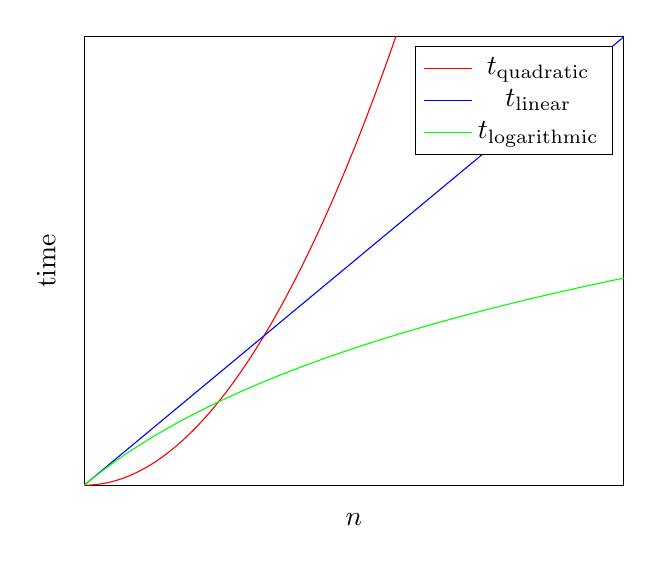
\begin{tikzpicture}
		\begin{axis}[ 
			xlabel=$n$,
			ylabel={time},
			xmin=0,
			ymin=0,
			xmax=3,
			ymax=3,
			yticklabels={,,},
			xticklabels={,,},
			tick style={draw=none}
			]
			\addplot[domain=0:3, samples=100, color=red]{x^2}; 
			\addlegendentry{\(t_{\mathrm{quadratic}}\)};
			 
			\addplot[domain=0:3, samples=100, color=blue]{x};
			\addlegendentry{\(t_{\mathrm{linear}}\)};
			
			\addplot[domain=0:3, samples=100, color=green]{ln(x+1)}; 
			\addlegendentry{\(t_{\mathrm{logarithmic}}\)};
		\end{axis}
	\end{tikzpicture}
\end{center}

We can see that logarithmic is the best scaling of the three, linear is worse, and quadratic is much worse.\\


% Course video 24
\subsection{Data Cleanup Algorithms\\ {\normalfont October 5, 2021}}
\bigbreak

The objective of these algorithms is to clean a dataset by removing undesirable items.\\

For example, you are making a survey about age. You ask 10 people ($n = 10$) and you get the following answers where 0 indicates missing data. 



\[
\renewcommand\arraystretch{1.5}
\begin{array}{|C|C|C|C|C|C|C|C|C|C|}\hline
	0 & 24 & 16 & 0 & 36 & 42 & 23 & 21 & 0 & 27 \\\hline
	\multicolumn{1}{c}{1} & \multicolumn{1}{c}{2} & \multicolumn{1}{c}{3} & \multicolumn{1}{c}{4} & \multicolumn{1}{c}{5} & \multicolumn{1}{c}{6} & \multicolumn{1}{c}{7} & \multicolumn{1}{c}{8} & \multicolumn{1}{c}{9} & \multicolumn{1}{c}{10}
\end{array}
\]\bigbreak

Let's say you want to find the average. If you take it directly, you would get that the average = $\frac{0+24+16+...+27}{10} = 18.9$ years. This is clearly not correct.\\

If instead you clean the data or account for the bad values, then you would get that the average = $\frac{24+16+...+27}{7} = 27$ years.\\

We will look at three data clean up algorithms:

\begin{itemize}
	\item The Shuffle Left
	\item The Copy-Over
	\item The Converging Pointers
\end{itemize}\bigbreak

% Course video 25, 26, 27
\subsubsection{The Shuffle Left Algorithm}
\bigbreak

The idea behind this algorithm is that it will
\begin{itemize}
	\item search the list from left to right
	\item If a zero is found, shuffle list to left
	\item It will also return the number of legitimate values in the list.
\end{itemize} 

You can imagine a school bus with students spread across the bus and the bus driver wants to get all students to move to the front end. He could start at the front of the bus and move down until he finds an empty seat. Once he finds an empty seat, he tells all students to shuffle forward. He can then look for the next empty seat, and repeat this until all the empty seats are in the back end of the bus.\\

For example, if we have the following list ($n = 6$)

\[
\renewcommand\arraystretch{1.5}
\begin{array}{|C|C|C|C|C|C|}\hline
	24 & 0 & 49 & 0 & 27 & 18 \\\hline
	\multicolumn{1}{c}{\color{green}\uparrow} & \multicolumn{1}{c}{\color{red}\uparrow} & \multicolumn{1}{c}{} & \multicolumn{1}{c}{} & \multicolumn{1}{c}{} & \multicolumn{1}{c}{}
\end{array}
\]\bigbreak

Let us define a pointer called Left (denoted in green) which indicates the index searching for zeros, and a pointer called Right (denoted in red) indicating position shuffle. We will also let Legit be the number of legit (here, non-zero) values. Initially, Left = 1, Right = 2, and Legit = $n$ = 6.\\

Now, we check if the value at position Left (green arrow) is legit, if it is, we increment Left and Right, so the list becomes:

\[
\renewcommand\arraystretch{1.5}
\begin{array}{|C|C|C|C|C|C|}\hline
	24 & 0 & 49 & 0 & 27 & 18 \\\hline
	\multicolumn{1}{c}{} & \multicolumn{1}{c}{\color{green}\uparrow} & \multicolumn{1}{c}{\color{red}\uparrow} & \multicolumn{1}{c}{} & \multicolumn{1}{c}{} & \multicolumn{1}{c}{}
\end{array}
\]\bigbreak

Now, we check if the value at position Left (green arrow) is legit, if it isn't we shuffle all values on the right of Left to the left and Legit is decremented. The list is now

\[
\renewcommand\arraystretch{1.5}
\begin{array}{|C|C|C|C|C|C|}\hline
	24 & 49 & 0 & 27 & 18 & 18 \\\hline
	\multicolumn{1}{c}{} & \multicolumn{1}{c}{\color{green}\uparrow} & \multicolumn{1}{c}{\color{red}\uparrow} & \multicolumn{1}{c}{} & \multicolumn{1}{c}{} & \multicolumn{1}{c}{}
\end{array}
\]\bigbreak

with Legit = 5. Note that the last value is duplicated. Also note that the Right pointer is used to do the shuffling. This process repeats.

\[
\renewcommand\arraystretch{1.5}
\begin{array}{|C|C|C|C|C|C|}\hline
	24 & 49 & 0 & 27 & 18 & 18 \\\hline
	\multicolumn{1}{c}{} & \multicolumn{1}{c}{} & \multicolumn{1}{c}{\color{green}\uparrow} & \multicolumn{1}{c}{\color{red}\uparrow} & \multicolumn{1}{c}{} & \multicolumn{1}{c}{}
\end{array}
\]\bigbreak

\[
\renewcommand\arraystretch{1.5}
\begin{array}{|C|C|C|C|C|C|}\hline
	24 & 49 & 27 & 18 & 18 & 18 \\\hline
	\multicolumn{1}{c}{} & \multicolumn{1}{c}{} & \multicolumn{1}{c}{\color{green}\uparrow} & \multicolumn{1}{c}{\color{red}\uparrow} & \multicolumn{1}{c}{} & \multicolumn{1}{c}{}
\end{array}
\]\bigbreak

And now Legit = 4. 

\[
\renewcommand\arraystretch{1.5}
\begin{array}{|C|C|C|C|C|C|}\hline
	24 & 49 & 27 & 18 & 18 & 18 \\\hline
	\multicolumn{1}{c}{} & \multicolumn{1}{c}{} & \multicolumn{1}{c}{} & \multicolumn{1}{c}{\color{green}\uparrow} & \multicolumn{1}{c}{\color{red}\uparrow} & \multicolumn{1}{c}{}
\end{array}
\]\bigbreak

Since Left = Legit, the algorithm halts.\\

Let's build the algorithm.

\begin{algorithm}
	\caption{Shuffle Left}
	\begin{algorithmic}[1]
		\Get $n, L_1, ..., L_n$
		\Set Legit = $n$
		\Set Left, Right = 1, 2
		\While{(Left $\le$ Legit)} step 5 to step 11
			\If{($L_{\mathrm{Left}}$ $\ne$ 0)}
				\Setx{2} Left = Left + 1
				\Setx{2} Right = Right + 1
			\Else
				\While{(Right $\leq$ Legit)} step 8 to 9
					\Set $L_{\mathrm{Right} - 1}$ = $L_{\mathrm{Right}}$
					\Set Right = Right + 1
				\EndWhile
				\Set Right = Left + 1
				\Set Legit = Legit - 1
			\EndIf
		\EndWhile
		\Stop
	\end{algorithmic}
\end{algorithm}


We will now do the complexity analysis.\\

\textbf{Best case scenario:} This occurs when there are no 0s in the list, since there are no shuffles. The number of iterations in this case is $n$. The complexity is $\Theta(n)$.\\

\textbf{Worst case scenario:} This occurs when the list entirely consists of 0s, since there are the maximum amount shuffles. The number of iterations in this case is $n - 1$ on the first shuffle, $n - 2$ on the second, etc. This means that the number of iterations is $1+2+3+...+(n-1) = \frac{n(n-1)}{2} = \frac{n^2}{2} - \frac{n}{2} \approx \frac{1}{2} n^2$. The complexity is $\Theta(n^2)$.\\


% Course video 28
\subsubsection{The Copy-Over Algorithm}
\bigbreak

The idea behind this algorithm is to scan the algorithm left to right and if a non-zero is found (legit), copy it into a new list.\\

For example, we will have the list L (size $n=8$) and we will move the legit values into the list newlist (size not yet known). We will make $i$ our pointer for iterating through L.

\[
\renewcommand\arraystretch{1.5}
\begin{array}{C|C|C|C|C|C|C|C|C|}\cline{2-9}
	L:~~~ & 23 & 0 & 45 & 42 & 0 & 0 & 2 & 7 \\\cline{2-9}
	\multicolumn{1}{c}{i} & \multicolumn{1}{c}{\uparrow} 
\end{array}
\]

\[
\renewcommand\arraystretch{1.5}
\begin{array}{C|CCCCC}\cline{2-6}
	newlist:~ & & & & & \\\cline{2-6}
\end{array}
\]\bigbreak

We can see that the first entry is non-zero, therefore, we put it into the newlist. We also increment $j$ which is a pointer for newlist.

\[
\renewcommand\arraystretch{1.5}
\begin{array}{C|C|C|C|C|C|C|C|C|}\cline{2-9}
	L:~~~ & 23 & 0 & 45 & 42 & 0 & 0 & 2 & 7 \\\cline{2-9}
	\multicolumn{1}{c}{i} & \multicolumn{1}{c}{\uparrow} 
\end{array}
\]

\[
\renewcommand\arraystretch{1.5}
\begin{array}{C|C|CCCC}\cline{2-6}
	newlist:~~~ & 23 & & & & \\\cline{2-6}
	\multicolumn{1}{c}{j} & \multicolumn{1}{c}{\uparrow}
\end{array}
\]\bigbreak

Then, we increment $i$ and repeat.

\[
\renewcommand\arraystretch{1.5}
\begin{array}{C|C|C|C|C|C|C|C|C|}\cline{2-9}
	L:~~~ & 23 & 0 & 45 & 42 & 0 & 0 & 2 & 7 \\\cline{2-9}
	\multicolumn{1}{c}{i} & \multicolumn{1}{c}{~} & \multicolumn{1}{c}{\uparrow} 
\end{array}
\]

\[
\renewcommand\arraystretch{1.5}
\begin{array}{C|C|CCCC}\cline{2-6}
	newlist:~~~ & 23 & & & & \\\cline{2-6}
	\multicolumn{1}{c}{j} & \multicolumn{1}{c}{\uparrow}
\end{array}
\]\bigbreak

Since $L_i$ is 0 here, we do not put that element in newlist (and we do not increment $j$). Instead, we simply increment $i$ and repeat.

\[
\renewcommand\arraystretch{1.5}
\begin{array}{C|C|C|C|C|C|C|C|C|}\cline{2-9}
	L:~~~ & 23 & 0 & 45 & 42 & 0 & 0 & 2 & 7 \\\cline{2-9}
	\multicolumn{1}{c}{i} & \multicolumn{1}{c}{~} & \multicolumn{1}{c}{~} & \multicolumn{1}{c}{\uparrow} 
\end{array}
\]

\[
\renewcommand\arraystretch{1.5}
\begin{array}{C|C|C|CCC}\cline{2-6}
	newlist:~~~ & 23 & 45 & & & \\\cline{2-6}
	\multicolumn{1}{c}{j} & \multicolumn{1}{c}{~} & \multicolumn{1}{c}{\uparrow}
\end{array}
\]\bigbreak

This whole process repeats until the lists and pointers look like this.

\[
\renewcommand\arraystretch{1.5}
\begin{array}{C|C|C|C|C|C|C|C|C|}\cline{2-9}
	L:~~~ & 23 & 0 & 45 & 42 & 0 & 0 & 2 & 7 \\\cline{2-9}
	\multicolumn{1}{c}{i} & \multicolumn{1}{c}{~} & \multicolumn{1}{c}{~} & \multicolumn{1}{c}{~} & \multicolumn{1}{c}{~} & \multicolumn{1}{c}{~} & \multicolumn{1}{c}{~} & \multicolumn{1}{c}{~} & \multicolumn{1}{c}{\uparrow} 
\end{array}
\]

\[
\renewcommand\arraystretch{1.5}
\begin{array}{C|C|C|C|C|C|}\cline{2-6}
	newlist:~~~ & 23 & 45 & 42 & 2 & 7 \\\cline{2-6}
	\multicolumn{1}{c}{j} & \multicolumn{1}{c}{~} & \multicolumn{1}{c}{~} & \multicolumn{1}{c}{~} & \multicolumn{1}{c}{~} & \multicolumn{1}{c}{\uparrow}
\end{array}
\]\bigbreak

\bigbreak Building the algorithm, we have


\begin{algorithm}
	\caption{Copy-Over}
	\begin{algorithmic}[1]
		\Get $n, L_1, ..., L_n$
		\Set i = 1
		\Set j = 1
		\While{(i $\le$ n)} step 5 to step 6
			\If{($L_i \ne 0$)}
				\Setx{2} $\mathrm{newlist}_j$ = $L_i$
				\Setx{2} j = j + 1
			\EndIf
			\Set i = i + 1
		\EndWhile
		\Stop
	\end{algorithmic}
\end{algorithm}\bigbreak


Now, for the complexity analysis.\\

There is no best or worse case scenarios in this algorithm. There is always $n$ iterations. That means that the \textbf{time complexity} is $\Theta(n)$.\\

Compared to the last algorithm, this is a much more efficient algorithm in time. However, the \textbf{space complexity} is worse. It requires double storage space.\\


\pagebreak
% Course video 29 and 30
\subsubsection{The Converging Pointers Algorithm}
\bigbreak

The idea behind this algorithm is that there are two pointers, Left and Right. 
\begin{itemize}
	\item Left moves up only if it is pointing at a non-zero value.
	\item If Left points at zero, copy the value at Right into Left and decrement Right by 1.
	\item Stop when Left = Right
\end{itemize}

For example, consider the following list (with $n = 8$). The blue arrow will represent the {\color{blue}Left} pointer and the red will represent the {\color{red}Right} pointer.

\[
\renewcommand\arraystretch{1.5}
\begin{array}{|C|C|C|C|C|C|C|C|}\hline
	0 & 24 & 16 & 0 & 23 & 21 & 0 & 27 \\\hline
	\multicolumn{1}{c}{\color{blue}\uparrow} & \multicolumn{1}{c}{~} & \multicolumn{1}{c}{~} & \multicolumn{1}{c}{~} & \multicolumn{1}{c}{~} & \multicolumn{1}{c}{~} & \multicolumn{1}{c}{~} & \multicolumn{1}{c}{\color{red}\uparrow}
\end{array}
\]\bigbreak

Notice that Left = 1 and Right = $n$ = 8. \\

Since the value at Left is 0, we put the value at Right into Left and decrement Right by 1. The list becomes

\[
\renewcommand\arraystretch{1.5}
\begin{array}{|C|C|C|C|C|C|C|C|}\hline
	27 & 24 & 16 & 0 & 23 & 21 & 0 & 27 \\\hline
	\multicolumn{1}{c}{\color{blue}\uparrow} & \multicolumn{1}{c}{~} & \multicolumn{1}{c}{~} & \multicolumn{1}{c}{~} & \multicolumn{1}{c}{~} & \multicolumn{1}{c}{~} & \multicolumn{1}{c}{\color{red}\uparrow} & \multicolumn{1}{c}{~}
\end{array}
\]\bigbreak

Now, Left moves forward until it is at a zero.

\[
\renewcommand\arraystretch{1.5}
\begin{array}{|C|C|C|C|C|C|C|C|}\hline
	27 & 24 & 16 & 0 & 23 & 21 & 0 & 27 \\\hline
	\multicolumn{1}{c}{~} & \multicolumn{1}{c}{~} & \multicolumn{1}{c}{~} & \multicolumn{1}{c}{\color{blue}\uparrow} & \multicolumn{1}{c}{~} & \multicolumn{1}{c}{~} & \multicolumn{1}{c}{\color{red}\uparrow} & \multicolumn{1}{c}{~}
\end{array}
\]\bigbreak

The entry at the Right pointer gets copied into the Left pointer and Right is decremented, giving

\[
\renewcommand\arraystretch{1.5}
\begin{array}{|C|C|C|C|C|C|C|C|}\hline
	27 & 24 & 16 & 0 & 23 & 21 & 0 & 27 \\\hline
	\multicolumn{1}{c}{~} & \multicolumn{1}{c}{~} & \multicolumn{1}{c}{~} & \multicolumn{1}{c}{\color{blue}\uparrow} & \multicolumn{1}{c}{~} & \multicolumn{1}{c}{\color{red}\uparrow} & \multicolumn{1}{c}{~} & \multicolumn{1}{c}{~}
\end{array}
\]\bigbreak

This process repeats until the pointers converge.

\[
\renewcommand\arraystretch{1.5}
\begin{array}{|C|C|C|C|C|C|C|C|}\hline
	27 & 24 & 16 & 21 & 23 & 21 & 0 & 27 \\\hline
	\multicolumn{1}{c}{~} & \multicolumn{1}{c}{~} & \multicolumn{1}{c}{~} & \multicolumn{1}{c}{\color{blue}\uparrow} & \multicolumn{1}{c}{\color{red}\uparrow} & \multicolumn{1}{c}{~} & \multicolumn{1}{c}{~} & \multicolumn{1}{c}{~}
\end{array}
\]\bigbreak

\[
\renewcommand\arraystretch{1.5}
\begin{array}{|C|C|C|C|C|C|C|C|}\hline
	27 & 24 & 16 & 21 & 23 & 21 & 0 & 27 \\\hline
	\multicolumn{1}{c}{~} & \multicolumn{1}{c}{~} & \multicolumn{1}{c}{~} & \multicolumn{1}{c}{~} & \multicolumn{1}{c}{{\color{blue}\uparrow}{\color{red}\uparrow}} & \multicolumn{1}{c}{~} & \multicolumn{1}{c}{~} & \multicolumn{1}{c}{~}
\end{array}
\]\bigbreak

The number of legit values is equal to the converged pointers. All of the legit values are to the left of the converged pointers. Note that this algorithm does not preserve order.\\

We can now build the algorithm.

\begin{algorithm}
	\caption{Converging Pointers}
	\begin{algorithmic}[1]
		\Get $n, L_1, ..., L_n$
		\Set Left = 1, Right = $n$
		\While{(Left $\le$ Right)} step 4 to step 5
			\If{($L_{\mathrm{Left}} \ne 0$)}
				\Setx{2} Left = Left + 1
			\Else
				\Setx{2} $L_{\mathrm{Left}}$ = $L_{\mathrm{Right}}$
				\Setx{2} Right = Right + 1
			\EndIf
		\EndWhile
		\Stop
	\end{algorithmic}
\end{algorithm}\bigbreak

We will now do the complexity analysis.\\

There is, again, no best or worse cases. The number of iterations is always $n$. Therefore, the complexity is $\Theta(n)$. 



\pagebreak
% Course video 31?
\subsection{Sorting Algorithms\\ {\normalfont October 13, 2021}}
\bigbreak


\subsubsection{Selection Sort}
\bigbreak


Let's say we have the list 

\[
\renewcommand\arraystretch{1.5}
\begin{array}{|C|C|C|C!{\color{red}\vline}}\hline
	2 & 15 & 8 & 7 \\\hline
	\multicolumn{1}{c}{~} & \multicolumn{1}{c}{\color{red}\uparrow} & \multicolumn{1}{c}{~} & \multicolumn{1}{c}{~}
\end{array}
\]\bigbreak

We scan the list and find the largest (denoted by the red arrow). We also start with a marker (red line) equal to the length of the list. Then, we swap the element at that index with the last element and decrement the marker. Then, we repeat on all elements before the marker.

\[
\renewcommand\arraystretch{1.5}
\begin{array}{|C|C|C!{\color{red}\vline}C|}\hline
	2 & 7 & 8 & 15 \\\hline
	\multicolumn{1}{c}{~} & \multicolumn{1}{c}{~} & \multicolumn{1}{c}{\color{red}\uparrow} & \multicolumn{1}{c}{~}
\end{array}
\]\bigbreak

\[
\renewcommand\arraystretch{1.5}
\begin{array}{|C|C!{\color{red}\vline}C|C|}\hline
	2 & 7 & 8 & 15 \\\hline
	\multicolumn{1}{c}{~} & \multicolumn{1}{c}{\color{red}\uparrow} & \multicolumn{1}{c}{~} & \multicolumn{1}{c}{~}
\end{array}
\]\bigbreak

\[
\renewcommand\arraystretch{1.5}
\begin{array}{|C!{\color{red}\vline}C|C|C|}\hline
	2 & 7 & 8 & 15 \\\hline
	\multicolumn{1}{c}{\color{red}\uparrow} & \multicolumn{1}{c}{~} & \multicolumn{1}{c}{~} & \multicolumn{1}{c}{~}
\end{array}
\]\bigbreak

\[
\renewcommand\arraystretch{1.5}
\begin{array}{!{\color{red}\vline}C|C|C|C|}\hline
	2 & 7 & 8 & 15 \\\hline
\end{array}
\]\bigbreak

The list is now sorted. The complexity of this algorithm is $\Theta(n^2)$. See Section \ref{selectionsort} for more details.


\subsubsection{Bubble Sort}
\bigbreak


Let's say we have the following list of size $n = 8$. 

\[
\renewcommand\arraystretch{1.5}
\begin{array}{|C|C|C|C|C|C|C|C|}\hline
	34 & 7 & 19 & 35 & 2 & 8 & 10 & 22\\\hline
	\multicolumn{1}{c}{\color{red}\uparrow} & \multicolumn{1}{c}{\color{blue}\uparrow} & \multicolumn{1}{c}{~} & \multicolumn{1}{c}{~} & \multicolumn{1}{c}{~} & \multicolumn{1}{c}{~} & \multicolumn{1}{c}{~} & \multicolumn{1}{c}{~}
\end{array}
\]\bigbreak

We start by comparing the first two elements with each other. If the element at the right (blue) arrow is larger than the left (red) one, then they swap. The red and blue counter advances. 

\[
\renewcommand\arraystretch{1.5}
\begin{array}{|C|C|C|C|C|C|C|C|}\hline
	7 & 34 & 19 & 35 & 2 & 8 & 10 & 22\\\hline
	\multicolumn{1}{c}{~} & \multicolumn{1}{c}{\color{red}\uparrow} & \multicolumn{1}{c}{\color{blue}\uparrow} & \multicolumn{1}{c}{~} & \multicolumn{1}{c}{~} & \multicolumn{1}{c}{~} & \multicolumn{1}{c}{~} & \multicolumn{1}{c}{~}
\end{array}
\]\bigbreak

This process repeats until the arrows reach the end of the list... 


\[
\renewcommand\arraystretch{1.5}
\begin{array}{|C|C|C|C|C|C|C|C|}\hline
	7 & 19 & 34 & 2 & 8 & 10 & 22 & 35\\\hline
	\multicolumn{1}{c}{~} & \multicolumn{1}{c}{~} & \multicolumn{1}{c}{~} & \multicolumn{1}{c}{~} & \multicolumn{1}{c}{~} & \multicolumn{1}{c}{~} & \multicolumn{1}{c}{\color{red}\uparrow} & \multicolumn{1}{c}{\color{blue}\uparrow}
\end{array}
\]\bigbreak


Now, we have ensured that the largest element in the list is at its final location. We can repeat the same process on all elements that are not sorted yet (at the moment, the first 7 elements). This takes $(n-1)$ iterations to do. After repeated the process once, the list will become

\[
\renewcommand\arraystretch{1.5}
\begin{array}{|C|C|C|C|C|C|C|C|}\hline
	7 & 19 & 2 & 8 & 10 & 22 & 34 & 35\\\hline
	\multicolumn{1}{c}{~} & \multicolumn{1}{c}{~} & \multicolumn{1}{c}{~} & \multicolumn{1}{c}{~} & \multicolumn{1}{c}{~} & \multicolumn{1}{c}{\color{red}\uparrow} & \multicolumn{1}{c}{\color{blue}\uparrow} & \multicolumn{1}{c}{~}
\end{array}
\]\bigbreak

This takes $(n-2)$ iterations to do. This repeats until we obtain the fully sorted list

\[
\renewcommand\arraystretch{1.5}
\begin{array}{|C|C|C|C|C|C|C|C|}\hline
	2 & 7 & 8 & 10 & 19 & 22 & 34 & 35\\\hline
	\multicolumn{1}{c}{\color{red}\uparrow} & \multicolumn{1}{c}{\color{blue}\uparrow} & \multicolumn{1}{c}{~} & \multicolumn{1}{c}{~} & \multicolumn{1}{c}{~} & \multicolumn{1}{c}{~} & \multicolumn{1}{c}{~} & \multicolumn{1}{c}{~}
\end{array}
\]\bigbreak

The total number of iterations this algorithm will take is $(n-1) + (n-2) + ... + 1 = \frac{n(n-1)}{2}$. This is a Gauss sum (minus $n$), so the complexity will be $\Theta(n^2)$ in the \textbf{worst case}.\\

In the \textbf{best case}, if we include a Boolean variable to the algorithm called "sorted" which is initially true and switches to false if a swap occurs. In that case, if the list is initially fully sorted, then the number of iterations is $n - 1$ and the complexity if $\Theta(n)$.\\


\subsubsection{Quick Sort}
\bigbreak

This algorithm uses a divide and conquer strategy. \\

Such a strategy works by the following steps:\\

\begin{itemize}
	\item Define a pivot
	\item Rearrange the list such that all elements that are less than the pivot are before it and all that are greater than the pivot come after it
	\item We now know that the picot is in the right location. We then apply this strategy on the left and right sub-lists.
\end{itemize}\bigbreak

Using the following list,

\[
\renewcommand\arraystretch{1.5}
\begin{array}{|C|C|C|C|C|C|C|C|}\hline
	34 & 2 & 15 & 7 & 33 & 9 & 20 & 4 \\\hline
\end{array}
\]\bigbreak


Where do we put the pivot?
\begin{itemize}
	\item Last element in the list
	\item First element in the list
	\item Median of sub-list
\end{itemize}

For our implementation, we will consider the first of these: Where the pivot (denoted by the red arrow) is initially at the last element in the list.\\

\[
\renewcommand\arraystretch{1.5}
\begin{array}{!{\color{green}\vline}C|C|C|C|C|C|C|C!{\color{green}\vline}}\arrayrulecolor{green}\hline
	34 & 2 & 15 & 7 & 33 & 9 & 20 & 4 \\\hline\arrayrulecolor{black}
	\multicolumn{1}{c}{~} & \multicolumn{1}{c}{~} & \multicolumn{1}{c}{~}  & \multicolumn{1}{c}{~} & \multicolumn{1}{c}{~} & \multicolumn{1}{c}{~} & \multicolumn{1}{c}{~} & \multicolumn{1}{c}{\color{red}\uparrow}
\end{array}
\]\bigbreak

Then, elements that are less than the pivot go to the left of the pivot, and elements that are greater than the pivot goes to the right.\\


\[
\renewcommand\arraystretch{1.5}
\begin{array}{!{\color{green}\vline}C!{\color{green}\vline}C!{\color{green}\vline}C|C|C|C|C|C!{\color{green}\vline}}\arrayrulecolor{green}\cline{1-1}\arrayrulecolor{black}\cline{2-3}\arrayrulecolor{green}\cline{3-8}\arrayrulecolor{black}
	2 & 4 & 34 & 15 & 7 & 33 & 9 & 20 \\\arrayrulecolor{green}\cline{1-1}\arrayrulecolor{black}\cline{2-3}\arrayrulecolor{green}\cline{3-8}\arrayrulecolor{black}
	\multicolumn{1}{c}{~} & \multicolumn{1}{c}{\color{red}\uparrow} & \multicolumn{1}{c}{~} & \multicolumn{1}{c}{~}  & \multicolumn{1}{c}{~} & \multicolumn{1}{c}{~} & \multicolumn{1}{c}{~} & \multicolumn{1}{c}{~}
\end{array}
\]\bigbreak

We know know that the pivot is in the correct position. We end up with two sub-lists now. Since the left sub-list is of size 1, we leave it as it is. And now we pick a pivot for the right sub-list (green boxes). We choose the rightmost element (20) and proceed with the algorithm. 

\[
\renewcommand\arraystretch{1.5}
\begin{array}{|C|C!{\color{green}\vline}C|C|C|C|C|C!{\color{green}\vline}}\arrayrulecolor{black}\cline{1-3}\arrayrulecolor{green}\cline{3-8}\arrayrulecolor{black}
	2 & 4 & 34 & 15 & 7 & 33 & 9 & 20 \\\arrayrulecolor{black}\cline{1-3}\arrayrulecolor{green}\cline{3-8}\arrayrulecolor{black}
	\multicolumn{1}{c}{~} & \multicolumn{1}{c}{~} & \multicolumn{1}{c}{~}  & \multicolumn{1}{c}{~} & \multicolumn{1}{c}{~} & \multicolumn{1}{c}{~} & \multicolumn{1}{c}{~} & \multicolumn{1}{c}{\color{red}\uparrow}
\end{array}
\]\bigbreak


\[
\renewcommand\arraystretch{1.5}
\begin{array}{|C|C!{\color{green}\vline}C|C|C!{\color{green}\vline}C!{\color{green}\vline}C|C!{\color{green}\vline}}\arrayrulecolor{black}\cline{1-3}\arrayrulecolor{green}\cline{3-6}\arrayrulecolor{black}\cline{6-7}\arrayrulecolor{green}\cline{7-8}\arrayrulecolor{black}
	2 & 4 & 15 & 7 & 9 & 20 & 34 & 33 \\\arrayrulecolor{black}\cline{1-3}\arrayrulecolor{green}\cline{3-6}\arrayrulecolor{black}\cline{6-7}\arrayrulecolor{green}\cline{7-8}\arrayrulecolor{black}
	\multicolumn{1}{c}{~} & \multicolumn{1}{c}{~} & \multicolumn{1}{c}{~}  & \multicolumn{1}{c}{~} & \multicolumn{1}{c}{~} & \multicolumn{1}{c}{\color{red}\uparrow} & \multicolumn{1}{c}{~} & \multicolumn{1}{c}{~}
\end{array}
\]\bigbreak


Now we repeat this on the new sub-lists.

\[
\renewcommand\arraystretch{1.5}
\begin{array}{|C|C!{\color{green}\vline}C|C|C!{\color{green}\vline}C!{\color{green}\vline}C|C!{\color{green}\vline}}\arrayrulecolor{black}\cline{1-3}\arrayrulecolor{green}\cline{3-6}\arrayrulecolor{black}\cline{6-7}\arrayrulecolor{green}\cline{7-8}\arrayrulecolor{black}
	2 & 4 & 15 & 7 & 9 & 20 & 34 & 33 \\\arrayrulecolor{black}\cline{1-3}\arrayrulecolor{green}\cline{3-6}\arrayrulecolor{black}\cline{6-7}\arrayrulecolor{green}\cline{7-8}\arrayrulecolor{black}
	\multicolumn{1}{c}{~} & \multicolumn{1}{c}{~} & \multicolumn{1}{c}{~}  & \multicolumn{1}{c}{~} & \multicolumn{1}{c}{\color{red}\uparrow} & \multicolumn{1}{c}{~} & \multicolumn{1}{c}{~} & \multicolumn{1}{c}{\color{red}\uparrow}
\end{array}
\]\bigbreak

\[
\renewcommand\arraystretch{1.5}
\begin{array}{|C|C!{\color{green}\vline}C!{\color{green}\vline}C!{\color{green}\vline}C!{\color{green}\vline}C|C!{\color{green}\vline}C!{\color{green}\vline}}\arrayrulecolor{black}\cline{1-3}\arrayrulecolor{green}\cline{3-4}\arrayrulecolor{black}\cline{4-5}\arrayrulecolor{green}\cline{5-6}\arrayrulecolor{black}\cline{6-7}\arrayrulecolor{green}\cline{8-8}\arrayrulecolor{black}
	2 & 4 & 7 & 9 & 15 & 20 & 33 & 34 \\\arrayrulecolor{black}\cline{1-3}\arrayrulecolor{green}\cline{3-4}\arrayrulecolor{black}\cline{4-5}\arrayrulecolor{green}\cline{5-6}\arrayrulecolor{black}\cline{6-7}\arrayrulecolor{green}\cline{8-8}\arrayrulecolor{black}
	\multicolumn{1}{c}{~} & \multicolumn{1}{c}{~} & \multicolumn{1}{c}{~}  & \multicolumn{1}{c}{\color{red}\uparrow} & \multicolumn{1}{c}{~} & \multicolumn{1}{c}{~} & \multicolumn{1}{c}{\color{red}\uparrow} & \multicolumn{1}{c}{~}
\end{array}
\]\bigbreak

Since all the sub-lists are of size one, the algorithm is finished and the sorted list is 

\[
\renewcommand\arraystretch{1.5}
\begin{array}{|C|C|C|C|C|C|C|C|}\hline
	2 & 4 & 7 & 9 & 15 & 20 & 33 & 34\\\hline
\end{array}
\]\bigbreak

As for the complexity, the \textbf{worse case} will happen when each pivot that is selected fails to divide the list. In this case, the complexity is $\Theta(n^2)$.\\

In the \textbf{best case}, we divide each list in half. In this case, the complexity is $\Theta(n \log_2n)$.\\



\section{Hardware}
\bigbreak

\subsection{Binary Numbering Systems}
\bigbreak
\subsubsection{Introduction and Definitions\\ {\normalfont October 13, 2021}}
\bigbreak

A \textbf{positional numbering system} of base $b$ and is given by

\begin{itemize}
	\item A natural number for the base $b$ (e.g. 2, 3, 4, 5, ...)
	\item A set of simple digits that contain $b$ digits (e.g. digits 0, 1, 2, ...,  ($b-1$))
	\item Position is used to determine the power of $b$ by which the digit is multiplied
\end{itemize}\bigbreak


A number in that numbering system is written as $(A)_b = A_mA_{m-1}...A_1A_0.A_{-1}A_{-2}...A_{-n}$. The part in front of the fractional dot is the \textit{integer part} and the part after is the \textit{fractional part}.\\

This is equivalent to $(A)_b = A_m\times b^m + A_{m-1}\times b^{m-1} + ... + A_1\times b^1 + A_0\times b^0 + A_{-1}\times b^{-1} + A_{-2}\times b^{-2} + ... + A_{-n}\times b^{-n}$.\\

If no base is specified, we assume that the base is base 10.\\

For example, $(4327)_{10} = 4 \times 10^3 + 3 \times 10^2 + 3 \times 10^1 + 7 \times 10^0 = 4327$.\\
Similarly, $(3.25)_{10} = 3 \times 10^0 + 2 \times 10^{-1} + 5 \times 10^{-2} = 3.25$.\\

Let's say now we have $(4021)_5$. By the formula above, 

\begin{align*}
	(4021)_5 &= 4 \times 5^3 + 0 \times 5^2 + 2 \times 5^1 + 1 \times 5^0\\
	&=  4 \times 125 + 0 \times 25 + 2 \times 5 + 1 \times 1\\
	&= (511)_{10}
\end{align*}\bigbreak


Another example, 

\begin{align*}
	(127.4)_5 &= 1 \times 5^2 + 2 \times 5^1 + 7 \times 5^0 + 4 \times 5^{-1}\\
	&=  1 \times 25 + 2 \times 5 + 7 \times 1 + \frac{4}{8}\\
	&= (87.5)_{10}
\end{align*}\bigbreak


In we write $(521)_4$, this is incorrect. This is because there is no digit 5 in base 4 (the only allowed symbols are 0, 1, 2, and 3).\\

The most frequent bases are decimal (base 10), binary (base 2), octal (base 8), and hexadecimal (base 16). Note that both octal and hexdecimal have bases that are powers of two ($8=2^3$ and $16=2^4$), so it is convenient to use for computers (since they run on binary).\\

For a binary example, 

\begin{align*}
	(11011.01)_2 &= 1 \times 2^4 + 1 \times 2^3 + 0 \times 2^2 + 1 \times 2^1 + 1 \times 2^0 + 0 \times 2^{-1} + 1 \times 2^{-2} \\
	&=  1 \times 16 + 1 \times 8 + 0 \times 4 + 1 \times 2 + 1 \times 1 + \frac{0}{2} + \frac{1}{4} \\
	&= (27.25)_{10}
\end{align*}\bigbreak

In binary, the allowed symbols are 0 and 1.\\
In octal, the allowed symbols are 0,1,2,3,4,5,6,7.\\
In hexadecimal, the allowed symbols are 0,1,2,3,4,5,6,7,8,9,A,B,C,D,E,F.\\

For a hexadecimal example,

\begin{align*}
	(\mathrm{B657})_{16} &= 11 \times 16^3 + 6 \times 16^2 + 5 \times 16^1 + 7 \times 16^0 \\
	&= (46687)_{10}
\end{align*}\bigbreak

Notice that hexadecimal is much more compact than in decimal or binary.\\


\subsubsection{Base conversion\\ {\normalfont October 13, 2021}}
\bigbreak

We have already converted from an arbitrary base to base 10. But how do we convert from base 10 to another base?\\

Starting with the \textit{integer part}, we will apply successive \textit{divisions} by the base and accumulate the remainders. \\

For example, if we want to convert $(53)_{10}$ to binary ($b=2$), we divide by 2 to get \textit{26} with a remainder of \textbf{1}. Then, we divide again by 2 to get \textit{13} with a remainder of \textbf{0}, again to get \textit{6} with remainder \textbf{1}, again to get \textit{3} with a remainder of \textbf{0}, again to get \textit{1} with a remainder of \textbf{1} and once more to get \textit{0} with a remainder of \textbf{1}. When we reach 0, we stop. Now, we accumulate the remainders (going \textbf{backwards}) to get that $(53)_{10} = (110101)_2$.\\

We can apply the same method to convert $(53)_{10}$ to octal, giving that $(53)_{10} = (65)_8$.\\

For the \textit{fractional part},we successively \textit{multiply} by the base and accumulate the integer parts.\\

For example, if we want to convert $(0.6875)_{10}$ to binary ($b = 2$), we multiply by 2 to get \textit{\textbf{1}.375}. We multiply the fractional part of the result by 2 again to get \textit{\textbf{0}.75}, again to get \textit{\textbf{1}.5}, and again to get \textit{\textbf{1}.0}. Since the fractional part is now 0, we stop. Now, we accumulate the integer parts (going \textbf{forwards}) to get that $(0.6875)_{10} = (0.1011)_2$.\\

\subsubsection{Octal \& Hexadecimal systems\\ {\normalfont October 13, 2021}}
\bigbreak

The following table shows the conversions between octal and binary.

\begin{center}
	\begin{table}[h]\centering
		\begin{tabular}{|c|c|}
			\hline
			Octal & Binary \\ \hline
			0     & 000     \\
			1     & 001     \\
			2     & 010     \\
			3     & 011     \\
			4     & 100     \\
			5     & 101     \\
			6     & 110     \\
			7     & 111    \\\hline
		\end{tabular}
	\end{table}\bigbreak
\end{center}

Using this table, we can easily convert, for example, $(562)_8$ to binary. It is simply $(562)_8 = (101~110~010)_2$. Similarly, we know that $(110~011~010~001)_2 = (6321)_8$.\\

We can use the same strategy for hexadecimal.

\begin{center}
	\begin{table}[h]\centering
		\begin{tabular}{|c|c|}
			\hline
			Hexadecimal & Binary \\ \hline
			0           & 0000   \\
			1           & 0001   \\
			2           & 0010   \\
			3           & 0011   \\
			4           & 0100   \\
			5           & 0101   \\
			6           & 0110   \\
			7           & 0111   \\
			8           & 1000   \\
			9           & 1001   \\
			A           & 1010   \\
			B           & 1011   \\
			C           & 1100   \\
			D           & 1101   \\
			E           & 1110   \\
			F           & 1111   \\ \hline
		\end{tabular}
	\end{table}
\end{center}

Using this table, we can easily convert, for example, $(\mathrm{5AB1})_{16}$ to binary. It is simply $(\mathrm{5AB1})_{16} = (0101~1010~1011~0001)_2$. Similarly, we know that $(1101~0111~1111)_2 = (\mathrm{D7F})_{16}$.\\

We use hexadecimal and octal because they are compact, and because conversion to/from binary is easier.\\

Hexadecimal is used to represent memory addresses. \\


\subsubsection{Binary Representation using a fixed number of bits\\ {\normalfont October 23, 2021}}
\bigbreak

In a computer, we use a \textbf{fixed} number of bits.\\

A \textbf{bit} stands for Binary Element. It is a binary digit. For example, 11 uses 2 bits, and 01101 uses 5 bits. A bit can be 0 or 1 and is difined by hardware.\\

Computer systems use a fixed number of bits to represent data. Most people use 64 bit computers nowadays. \\

For example, if we have an 8 bit computer system, then we can convert the decimals to binary as follows.

\[
\renewcommand\arraystretch{1.5}
\begin{array}{C|C|C|C|C|C|C|C|C|}\cline{2-9}
	(3)_{10} & 0 & 0 & 0 & 0 & 0 & 0 & 1 & 1\\\cline{2-9}
	(15)_{10} & 0 & 0 & 0 & 0 & 1 & 1 & 1 & 1\\\cline{2-9}
	(255)_{10} & 1 & 1 & 1 & 1 & 1 & 1 & 1 & 1\\\cline{2-9}
	\multicolumn{1}{c}{~} & \multicolumn{1}{c}{\color{blue}\uparrow} & \multicolumn{1}{c}{~} & \multicolumn{1}{c}{~}  & \multicolumn{1}{c}{~} & \multicolumn{1}{c}{~} & \multicolumn{1}{c}{~} & \multicolumn{1}{c}{~} & \multicolumn{1}{c}{\color{red}\uparrow}
\end{array}
\]\bigbreak

We call the leftmost bit (blue arrow) the Most Significant Bit (MSB), and the rightmost bit (red arrow) is called the Least Significant Bit (LSB).\\

For 8 bits, the smallest integer is $(0)_{10} = (0000~0000)_{2}$ and the largest integer is $(255)_{10} = (1111~1111)_{2} = (256 - 1)_{10} = (2^8 - 1)_{10}$. \\

In general for $n$ bits, the smallest integer is $(0)_{10}$ and the largest integer is $(2^n - 1)_{10}$. This gives $2^n$ available integers.\\


\subsection{Representation of Signed Integers}
\bigbreak

\textbf{Signed integers} are integers that have the possibility of being negative. For example, +6, -3, +51, and -23 are all signed integers. A negative integer is a signed integer, but a signed integer is not necessarily a negative number. There are a couple representations for signed numbers in a computer.\\

\subsubsection{Signed magnitude representation}
\bigbreak

The MSB is used for the sign (+ or -) and the rest is the magnitude. By convention, the + is represented by a 0 and the - is represented by a 1.

\[
\renewcommand\arraystretch{1.5}
\begin{array}{C|C|C|C|C|C|C|C|C|}\cline{2-9}
	(+6)_{10} & 0 & 0 & 0 & 0 & 0 & 1 & 1 & 0\\\cline{2-9}
	(-6)_{10} & 1 & 0 & 0 & 0 & 0 & 1 & 1 & 0\\\cline{2-9}
	(-127)_{10} & 1 & 1 & 1 & 1 & 1 & 1 & 1 & 1\\\cline{2-9}
\end{array}
\]\bigbreak

The smallest number for an 8 bit computer in this representation is $(-127)_{10} = 1111~1111$ and the largest is $(+127)_{10} = 0111~1111$. There are 256 representations. Note, however, that there are two zeros ($(-0)_{10} = 1000~0000$ and $(+0)_{10} = 0000~0000$)... This is an issue. \\

In general, for an $n$ bit computer in the signed magnitude representation, there are 2 zeros, $2^{n-1} - 1$ negative numbers and $2^{n-1} - 1$ positive numbers. There are $2^n$ representations.\\

To show that we have a problem with this representation system, we will assume a 3-bit computer system. 

\begin{center}
	\begin{table}[h]\centering
		\begin{tabular}{|c|c|c|}
			\hline
			Binary & (Unsigned integers)$_{10}$ & (Signed integers)$_{10}$ \\ \hline
			000 & 0 & +0 \\
			001 & 1 & +1 \\
			010 & 2 & +2 \\
			011 & 3 & +3 \\
			100 & 4 & -0 \\
			101 & 5 & -1 \\
			110 & 6 & -2 \\
			111 & 7 & -3 \\ \hline
		\end{tabular}
	\end{table}
\end{center}

The \textit{first issue} here is that there are two zeros, but zero should not have a sign.\\

The \textit{second issue} has to do with integer addition. We can write that $5 - 2 = (+5) + (-2)$. Thus, we can use signed integers and addition to do subtraction of any numbers. Let's say we want to do $1 - 3 = (+1) + (-3) = (-2)$ in binary. We can write this as follows\\

\begin{center}
	\begin{tabular}{cccc}
		\tiny 1& \tiny 1 & \tiny 1 &  \\
		& 0 & 0 & 1 \\
		+ & 1  & 1 & 1 \\
		\hline
		1 & 0 & 0 & 0 \\
	\end{tabular}
	\bigbreak
\end{center}

Typically, a computer will cut off the leftmost bit to make it 3 bits long to give an answer of $(000)_2 = (+0)_{10}$. In principle, we should get $(-2)_{10} = (110)_2$, which is not what we get. There is our second issue with this representation: signed magnitude does not allow arthritic operations.\\ 

We need to use another representation to fix these problems.\\

\subsubsection{The 2's complement}
\bigbreak

First we will define the \textbf{1's complement}: The 1's complement of a binary number is obtained by complementing (taking the opposite) of each binary digit in the number. For example, the 1's complement of 0 is 1, of 1 is 0, of 001 is 110, of 11011 is 00100. \\

Note that if you add a binary number to it's 1's complement, you will always get a number of the same size, consisting only of 1s.\\

The \textbf{2's complement} is found by first taking the 1's complement and then adding 1. For example, the 2's complement of 1011 is 0100 + 1 = 0101, and of 110101 is 001010 + 1 = 001011. \\

Note that if you add a binary number to it's 2's complement, you will always get a number of the size, consisting of 1s, plus another bit to the left that is 1 (carry). If we cut off the carry, then we get 0. Therefore, the opposite sign can be given by the 2's complement (since the sum is 0).\\

Thus, we conclude that we can use the 2's complement represents signed numbers. If you take the 2's complement on a positive number, it will give you the equivalent negative number and vice versa.\\


\subsubsection{2's complement representation}
\bigbreak

The following is a conversion table comparing this representation to the signed magnitude representation.

\begin{center}
	\begin{table}[h]\centering
		\begin{tabular}{|c|c|c|c|}
			\hline
			Binary & (Unsigned integers)$_{10}$ & (Signed magnitude)$_{10}$ & (2's complement)$_{10}$ \\ \hline
			000 & 0 & +0 & +0\\
			001 & 1 & +1 & +1\\
			010 & 2 & +2 & +2\\
			011 & 3 & +3 & +3\\
			100 & 4 & -0 & -4\\
			101 & 5 & -1 & -3\\
			110 & 6 & -2 & -2\\
			111 & 7 & -3 & -1\\ \hline
		\end{tabular}
	\end{table}
\end{center}

With the 2's complement representation, we solve the double zero issue. Now, we will check if arthritic operations work in this representation. We will add (+1) + (-3). 

\begin{center}
	\begin{tabular}{cccc}
		\tiny & \tiny  & \tiny 1 &  \\
		& 0 & 0 & 1 \\
		+ & 1  & 0 & 1 \\
		\hline
		& 1 & 1 & 0 \\
	\end{tabular}
	\bigbreak
\end{center}

We indeed do get $(110)_2 = (-2)_{10}$ as expected.

\subsubsection{Comprehensive example and other representations}
\bigbreak

Consider an 8 bit system. Assume that the following is stored in memory:  A = 10100110 .\\

What is A?\\

We need a representation to answer this question. We will compute it for each of the representations we know (unsigned, signed magnitude, and 2's complement representations).\\

\textbf{Unsigned}: $(2 + 4 + 32 + 128)_{10} = (166)_{10}$\\

\textbf{Signed magnitude}: $-(2 + 4 + 32)_{10} = (-38)_{10}$\\

\textbf{2's complement}: $-(01011001 + 1)_2 = -(01011010)_2 = -(2 + 8 + 16 + 64)_{10} = (-92)_{10}$\\

Your program decides which representation to use.\\

We can also use a number to represent a pixel on an image. If we use gray scale in an 8-bit computer system, we can represent the different shades by binary numbers. By convention, we let a black pixel be $(0)_{10} = (0000~0000)_2$ and a white pixel be $(255)_{10} = (1111~1111)_2$. Therefore, for an 8-bit system, there are 256 possible shades. If we want to represent color, we use 3 binary numbers that represent the red, green and blue parts of the color (RGB).\\

For text, a common encoding (representation) is ASCII code. There is a table that converts an 8-bit binary number to an ASCII character. 


\subsection{Boolean Logic}
\bigbreak

\textbf{Boolean logic} is a branch of mathematics developed by George Boole. Boolean logic manipulates \textit{Boolean data} using \textit{Boolean operators}.\\

A \textbf{Boolean variable} takes only two possible values $\in$ \{True, False\} (\{1, 0\} respectively).\\
	
A \textbf{Boolean (logic) operators} take a Boolean as input and result in a Boolean. The basic operators are AND, OR, and NOT.\\


\subsubsection{AND operator}
\bigbreak
Let a, b, c be Boolean variables. We define c = a AND b = a$\cdot$b = ab. The following is the \textbf{truth table} for this operation.\\

\begin{center}
	\begin{tabular}{|c|c|c|}
		a & b & c = ab \\\hline
		0 & 0  & 0 \\
		0 & 1  & 0 \\
		1 & 0  & 0 \\
		1 & 1  & 1 \\
	\end{tabular}
	\bigbreak
\end{center}

Sometimes the AND operation is called the \textit{min operator} because it takes the minimum of the two values.\\

A \textbf{logic gate} is an electronic circuit that implements a Boolean operation. The AND gate is represented as follows:\\

\begin{center}
	\begin{circuitikz}\draw
		(0, 0) node[and port] (myand1) {}
		(-2cm, +0.3cm) node[anchor=south]{a} -- (myand1.in 1)
		(-2cm, -0.3cm) node[anchor=north]{b} -- (myand1.in 2)
		(myand1.out) -- (+0.5cm, 0) node[anchor=north]{c};
	\end{circuitikz}
\end{center}\bigbreak

In a logic gate, logic 1 corresponds to 5 Volts and logic 0 corresponds to 0 Volts.\\

\subsubsection{OR operator}
\bigbreak
Let a, b, c be Boolean variables. We define c = a OR b = a + b. The following is the \textbf{truth table} for this operation.\\

\begin{center}
	\begin{tabular}{|c|c|c|}
		a & b & c = a + b \\\hline
		0 & 0  & 0 \\
		0 & 1  & 1 \\
		1 & 0  & 1 \\
		1 & 1  & 1 \\
	\end{tabular}
	\bigbreak
\end{center}

Sometimes the OR operation is called the \textit{max operator} because it takes the maximum of the two values.\\

The OR logic gate is represented as follows:\\

\begin{center}
	\begin{circuitikz}\draw
		(0, 0) node[or port] (myor1) {}
		(-2cm, +0.3cm) node[anchor=south]{a} -- (myor1.in 1)
		(-2cm, -0.3cm) node[anchor=north]{b} -- (myor1.in 2)
		(myor1.out) -- (+0.5cm, 0) node[anchor=north]{c};
	\end{circuitikz}
\end{center}\bigbreak


\subsubsection{NOT operator}
\bigbreak
Let a, c be Boolean variables. We define c = NOT a = $\bar{a}$ = a`. The following is the \textbf{truth table} for this operation.\\

\begin{center}
	\begin{tabular}{|c|c|}
		a & c = $\bar{a}$ \\\hline
		0 & 1  \\
		1 & 0  \\
	\end{tabular}
	\bigbreak
\end{center}

The OR logic gate is represented as follows:\\

\begin{center}
	\begin{circuitikz}\draw
		(0, 0) node[not port] (mynot1) {}
		(-1cm, 0) node[anchor=south]{a} -- (mynot1.in)
		(mynot1.out) -- (+1cm, 0) node[anchor=north]{c};
	\end{circuitikz}
\end{center}\bigbreak

\subsubsection{Properties of Operators}
\bigbreak

The AND and OR operators are associative: \\
$(x \cdot y) \cdot z = x \cdot (y \cdot z)$ and $(x + y) + z = x + (y + z)$.\\

The AND and OR operators are commutative: \\
$x \cdot y = y \cdot x$ and $x + y = y + x$.\\

The AND and OR operators are distributive: \\
$x \cdot (y + z) = x \cdot y + x \cdot z$\\


The AND and OR operators have identity and zero values: \\
$x \cdot 1 = x$ and $x \cdot 0 = 0$\\
$x + 0 = x$ and $x + 1 = 1$\\
$x \cdot x` = 0$ and $x + x` = 1$\\


\subsubsection{De Morgan Theorem}
\bigbreak

De Morgan's Theorem states that\\

$(x + y)` = x` \cdot y`$\\
$(x \cdot y)` = x` + y`$\\

We will use truth tables to proof this theorem.\\

Starting with the $(x + y)` = x` \cdot y`$ case:\\

\begin{center}
	\begin{tabular}{|c|c|c|c|c|c|c|}
		x & y & (x+y) & (x+y)` & x` & y` & x` $\cdot$ y` \\\hline
		0 & 0 & 0 & 1 & 1 & 1 & 1 \\
		0 & 1 & 1 & 0 & 1 & 0 & 0 \\
		1 & 0 & 1 & 0 & 0 & 1 & 0 \\
		1 & 1 & 1 & 0 & 0 & 0 & 0 \\
	\end{tabular}
	\bigbreak
\end{center}

Notice that the (x+y)` and x` $\cdot$ y` columns are identical.\\

Now for the $(x \cdot y)` = x` + y`$ case:\\

\begin{center}
	\begin{tabular}{|c|c|c|c|c|c|c|}
		x & y & (x$\cdot$y) & (x$\cdot$y)` & x` & y` & x` + y` \\\hline
		0 & 0 & 0 & 1 & 1 & 1 & 1 \\
		0 & 1 & 0 & 1 & 1 & 0 & 1 \\
		1 & 0 & 0 & 1 & 0 & 1 & 1 \\
		1 & 1 & 1 & 0 & 0 & 0 & 0 \\
	\end{tabular}
	\bigbreak
\end{center}

Notice that the (x$\cdot$y)` and x` + y` columns are identical.\\

Thus, the de Morgan Theorem is proved.\\


\subsubsection{Boolean functions}

A \textbf{Boolean function} is a combination of multiple Boolean variables using multiple Boolean operators to obtain a Boolean output.\\

We express Boolean functions with: A Boolean expression, a truth table, a logic diagram (logic gates).\\

For example, let's express $f_1 = a \cdot b \cdot c$ in three ways. It is already expressed as a Boolean expression. Let's construct a truth table:

\begin{center}
	\begin{tabular}{|c|c|c|c|}
		a & b & c & $f_1$ \\\hline
		0 & 0 & 0 & 0 \\
		0 & 0 & 1 & 0 \\
		0 & 1 & 0 & 0 \\
		0 & 1 & 1 & 0 \\
		1 & 0 & 0 & 0 \\
		1 & 0 & 1 & 0 \\
		1 & 1 & 0 & 0 \\
		1 & 1 & 1 & 1 \\
	\end{tabular}
	\bigbreak
\end{center}

Representing this in a logic diagram, we get

\begin{center}
	\begin{circuitikz}\draw
		(0, 0) node[and port] (myand1) {}
		(3cm, -0.3cm) node[and port] (myand2) {}
		(-2cm, +0.3cm) node[anchor=north]{a} -- (myand1.in 1)
		(-2cm, -0.3cm) node[anchor=north]{b} -- (myand1.in 2)
		(myand1.out) -- (myand2.in 1)
		(-2cm, -0.9cm) node[anchor=north]{c} -| (0.5cm, -0.9cm) |- (myand2.in 2)
		(myand2.out) -- (3.5cm, -0.3cm) node[anchor=north]{$f_1$};
	\end{circuitikz}
\end{center}\bigbreak


A second example is with $f_2 = (a + b) \cdot \bar{c}$. The truth table of $f_2$ is

\begin{center}
	\begin{tabular}{|c|c|c|c|c|}
		a & b & c & a+b & $f_2$ \\\hline
		0 & 0 & 0 & 0 & 0 \\
		0 & 0 & 1 & 0 & 0 \\
		0 & 1 & 0 & 1 & 1 \\
		0 & 1 & 1 & 1 & 0 \\
		1 & 0 & 0 & 1 & 1 \\
		1 & 0 & 1 & 1 & 0 \\
		1 & 1 & 0 & 1 & 1 \\
		1 & 1 & 1 & 1 & 0 \\
	\end{tabular}
	\bigbreak
\end{center}

The logic diagram is

\begin{center}
	\begin{circuitikz}\draw
		(0, 0) node[or port] (myor) {}
		(-0.5cm, -1.5cm) node[not port] (mynot) {}
		(3cm, -0.3cm) node[and port] (myand) {}
		(-2cm, +0.3cm) node[anchor=north]{a} -- (myor.in 1)
		(-2cm, -0.3cm) node[anchor=north]{b} -- (myor.in 2)
		(myor.out) -- (myand.in 1)
		(-2cm, -1.5cm) node[anchor=north]{c} -- (mynot.in) 
		(mynot.out) -| (0.5cm, -0.9cm) |- (myand.in 2)
		(myand.out) -- (3.5cm, -0.3cm) node[anchor=north]{$f_2$};
	\end{circuitikz}
\end{center}\bigbreak

Question 1: Is the Boolean expression unique for a given function? No! Since $f_2 = (a + b) \cdot \bar{c} = a \cdot \bar{c} + b \cdot \bar{c}$.\\

Question 2: Is the diagram unique? No! As above, you can make the diagram be such that $f_2 = a \cdot \bar{c} + b \cdot \bar{c}$. Namely, 

\begin{center}
	\begin{circuitikz}\draw
		(0, 0) node[and port] (myand1) {}
		(0, -1.5cm) node[and port] (myand2) {}
		(3cm, -0.3cm) node[or port] (myor) {}
		(-2.8cm, -0.75cm) node[not port] (mynot) {}
		
		(-4cm, +0.3cm) node[anchor=north]{a}-- (myand1.in 1)
		(-4cm, -0.75cm) node[anchor=north]{c} -- (mynot.in)
		(-4cm, -1.8cm) node[anchor=north]{a}-- (myand2.in 2)
		
		(myand1.out) -- (myor.in 1)
		(mynot.out) -- (myand1.in 2)
		(mynot.out) -- (myand2.in 1)
		(myand2.out) -| (0.5cm, -0.9cm) |- (myor.in 2)
		(myor.out) -- (3.5cm, -0.3cm) node[anchor=north]{$f_2$};
	\end{circuitikz}
\end{center}\bigbreak

Question 3: Is the truth table unique? Yes! Always, since we use the truth table to define when two Boolean functions are equal.\\

A third example could be $f_3 = ab + \bar{a}\bar{b}$. The following is the truth table.

\begin{center}
	\begin{tabular}{|c|c|c|c|c|}
		a & b & ab & $\bar{a}\bar{b}$ & $f_2$ \\\hline
		0 & 0 & 0 & 1 & 1 \\
		0 & 1 & 0 & 0 & 0 \\
		1 & 0 & 0 & 0 & 0 \\
		1 & 1 & 1 & 0 & 1 \\
	\end{tabular}
	\bigbreak
\end{center}

The logic diagram is

\begin{center}
	\begin{circuitikz}\draw
		(7cm, 0) node[or port] (myor) {}
		(5cm, 1.5cm) node[and port] (myand1) {}
		(5cm, -1.5cm) node[and port] (myand2) {}
		(1.6cm, 0.75cm) node[not port] (mynot1) {}
		(1.6cm, -1.8cm) node[not port] (mynot2) {}
		
		(0, 1.79cm) node[anchor=north]{a} -- (myand1.in 1)
		(0, 1.79cm) -| (mynot1.in)
		(0, -0.44cm) node[anchor=north]{b} -| (myand1.in 2)
		(0, -0.44cm) -| (mynot2.in)
		
		(mynot1.out) -- (myand2.in 1)
		(mynot2.out) -- (myand2.in 2)
		
		(myand1.out) -- (myor.in 1)
		(myand2.out) -- (myor.in 2)
		(myor.out) -- (7.5cm, 0cm) node[anchor=north]{$f_3$};
	\end{circuitikz}
\end{center}\bigbreak


In a fourth example, we will consider $F_1 = x'y'z + x'yz + xy'$ and $F_2 = x'z + xy'$. We will prove that they are identical and show each of their logic diagrams.\\

We can show that $F_1$ and $F_2$ are identical by checking their truth table results, however we will show it using Boolean properties.\\

Since $F_1$ has more terms than $F_2$, we will try to convert $F_1$ to $F_2$.

\begin{align*}
	F_1 &= x'y'z + x'yz + xy'\\
	&= x'z(y'+ y) + xy'\\
	&= x'z(1) + xy'\\
	&= x'z+xy'\\
	&= F_2
\end{align*}\bigbreak

Now we will show the logic diagram of $F_1$.

\begin{center}
	\begin{circuitikz}\draw
		% ---- INPUTS -----
		(0, 2cm) node[anchor=north]{x} node[](x){}
		(0, 0cm) node[anchor=north]{y} node[](y){}
		(0, -2cm) node[anchor=north]{z} node[](z){}
		%nots
		(x) ++ (1.5cm, -1cm) node[not port, scale=0.75] (notx) {}
		(y) ++ (1.5cm, -1cm) node[not port, scale=0.75] (noty) {}
	
		%not-links
		(x) ++ (1cm, 0) node[](notxlink){} to[short, *-] (notx.in) 
		(x) -- ++ (1cm, 0) (notxlink)
		(y) ++ (1cm, 0) node[](notylink){} to[short, *-] (noty.in) 
		(y) -- ++ (1cm, 0) (notylink)
		
		(x) -- ++ (2.25cm, 0)
		(y) -- ++ (2.25cm, 0)
		(z) -- ++ (2.5cm, 0)
		
		% ----- GATES -----
		(4.5cm, 2cm) node[and port] (and1) {}
		(4.5cm, 0cm) node[and port] (and2) {}
		(4.5cm, -2cm) node[and port] (and3) {}
		(7cm, 2cm) node[and port] (and21) {}
		(7cm, 0cm) node[and port] (and22) {}
		(9cm, 1cm) node[or port] (or1) {}
		(11cm, 0cm) node[or port] (or2) {}
		
		%connections
		(notx.out) -- ++(0.5cm, 0) |- (and1.in 1)
		(noty.out) -- ++(0.25cm, 0) |- (and1.in 2)
		
		(notx.out) -- ++(0.5cm, 0) |- (and2.in 1)
		(y) ++ (2.25cm, 0) -- ++(0.3cm, 0) |- (and2.in 2)
		
		(x) ++ (2.25cm, 0) -- ++(0.75cm, 0) |- (and3.in 1)
		(noty.out) -- ++(0.25cm, 0) |- (and3.in 2)
		
		(and1.out) -- ++ (0.2cm, 0) |- (and21.in 1)
		(z) ++ (2.5cm, 0) -- ++ (0, 1cm) -- ++ (2.35cm, 0) |- (and21.in 2)
		
		(and2.out) -- ++ (0.6cm, 0) |- (and22.in 1)
		(z) ++ (2.5cm, 0) -- ++ (0, 1cm) -- ++ (2.5cm, 0) -- ++ (0.3cm, 0) |- (and22.in 2)
		
		(and21.out) -- ++ (0.3cm, 0) |- (or1.in 1)
		(and22.out) -- ++ (0.3cm, 0) |- (or1.in 2)
		
		(or1.out) -- ++ (0.3cm, 0) |- (or2.in 1)
		(and3.out) -- ++ (3cm, 0) |- (or2.in 2)
		
		% ----- OUTPUT -----
		(11.5cm, 0cm) node[anchor=north]{$F_1$};
	\end{circuitikz}
\end{center}\bigbreak\bigbreak



And the logic diagram of $F_2$ is

\begin{center}
	\begin{circuitikz}\draw
		% ---- INPUTS -----
		(0, 2cm) node[anchor=north]{x} node[](x){}
		(0, 0cm) node[anchor=north]{y} node[](y){}
		(0, -2cm) node[anchor=north]{z} node[](z){}
		%nots
		(x) ++ (1.5cm, -1cm) node[not port, scale=0.75] (notx) {}
		(y) ++ (1.5cm, -1cm) node[not port, scale=0.75] (noty) {}
		
		%not-links
		(x) ++ (1cm, 0) node[](notxlink){} to[short, *-] (notx.in) 
		(x) -- ++ (1cm, 0) (notxlink)
		(y) ++ (1cm, 0) node[](notylink){} to[short, *-] (noty.in) 
		(y) -- ++ (1cm, 0) (notylink)
		
		(x) -- ++ (2.25cm, 0)
		(z) -- ++ (2.25cm, 0)
		
		% ----- GATES -----
		(5cm, 1cm) node[and port] (and1) {}
		(5cm, -1cm) node[and port] (and2) {}
		(7cm, 0cm) node[or port] (or) {}
		
		%connections
		(x) ++ (2.25cm, 0) -- ++(1cm, 0) |- (and1.in 1)
		(noty.out) -- ++(1.2cm, 0) |- (and1.in 2)
		
		(notx.out) -- ++(0.75cm, 0) |- (and2.in 1)
		(z) -- ++ (2.75cm, 0) |- (and2.in 2)
		
		(and1.out) -- (or.in 1)
		(and2.out) -- (or.in 2)
		
		% ----- OUTPUT -----
		(7.5cm, 0cm) node[anchor=north]{$F_1$};
	\end{circuitikz}
\end{center}\bigbreak\bigbreak

The following are a few examples of simplifying Boolean expressions:

\begin{align*}
	x(x'+y)&=xx'+xy\\
	&= 0+ xy\\
	&= xy
\end{align*}\bigbreak

\begin{align*}
	(x+y)(x+y') &= xx + xy' + xy + yy'\\
	&= x+x(y'+y)+0\\
	&= x+x(1)\\
	&= x+x\\
	&= x
\end{align*}\bigbreak

\begin{align*}
	((x+y)(x+y'))' &= (x+y)' + (x+y')'\\
	&= x'y'+x'y\\
	&= x'(y'+y)\\
	&= x'(1)\\
	&= x'
\end{align*}\bigbreak


\subsubsection{Boolean Expression from Truth Table}

So far, we have been given a Boolean expression and have been told to generate a truth table and implement it in a logic diagram. If instead, we start with the logic diagram, it is not hard to find the Boolean expression and the truth table. However, if we are given a truth table, it is not as straightforward. If we can get the Boolean Expression from the truth table, getting the logic diagram is easy. So the question is: \textit{How do we get a Boolean expression from a truth table?}\\

Let's assume a function $f(x, y)$ that has the truth table

\begin{center}
	\begin{tabular}{|c|c||c|}
		a & b & $f$ \\\hline
		0 & 0 & 0 \\
		0 & 1 & 0 \\
		1 & 0 & 1 \\
		1 & 1 & 1 \\
	\end{tabular}
	\bigbreak
\end{center}

We know that $f=1$ when ($x=1$ AND $y=0$) OR when ($x=1$ AND $y=1$). Simplifying, $f=1$ when $x\bar{y} + xy$. Checking the truth table, this works for all values. Thus, the function is $f = x(\bar{y} + y) = x(1) = x$.\\

Let's now assume a function $f_2(x, y)$ that has the truth table

\begin{center}
	\begin{tabular}{|c|c||c|}
		a & b & $f_2$ \\\hline
		0 & 0 & 0 \\
		0 & 1 & 1 \\
		1 & 0 & 1 \\
		1 & 1 & 0 \\
	\end{tabular}
	\bigbreak
\end{center}

We will look at all values of $f=1$ and find the combination of $x$ and $y$ that make $f=1$. In this case, we know that $f=1$ when ($x=0$ AND $y=1$) OR when ($x=1$ AND $y=0$). Simplifying, $f=1$ when $\bar{x} + x\bar{y}$.\\

We say that $f$ is written as a \textbf{sum of products} (OR of ANDs). This is also called the \textbf{canonical form}.\\

Let's do a larger example: Express the following using the sum of products. 

\begin{center}
	\begin{tabular}{|c|c|c||c|}
		x & y & z & $f_3$ \\\hline
		0 & 0 & 0 & 0\\
		0 & 0 & 1 & 0\\
		0 & 1 & 0 & 1\\
		0 & 1 & 1 & 1\\
		1 & 0 & 0 & 0\\
		1 & 0 & 1 & 0\\
		1 & 1 & 0 & 1\\
		1 & 1 & 1 & 1\\
	\end{tabular}
	\bigbreak
\end{center}

For the first time $f=1$, we get $\bar{x}y\bar{z}$, then $\bar{x}yz$, and so on. In the end, we get that $f = \bar{x}y\bar{z} + \bar{x}yz + xy\bar{z} + xyz$. This simplifies to just $f=y$. \\


\subsection{Combinational Logic Circuits}

A \textbf{logic circuit} is a circuit that 

\begin{itemize}
	\item Takes $n$ binary inputs
	\item Transforms inputs using logic gates
	\item Produce $m$ binary outputs
\end{itemize}\bigbreak

When we say that a logic circuit is \textbf{combinational}, we mean that the outputs at a given time $t$ depend only on the inputs at time $t$. In other words, there is no notion of what the circuit has done in the past nor what it will do in the future.\\

The opposite of a combinational logic circuit is a \textbf{sequential} logic circuit that \textit{does} depend on time. An example of a sequential logic circuit is an a digital clock.\\

If a logic circuit has $n$ inputs, it has $2^n$ possible combinations of binary input.\\

The steps that one must follow in order to build a combinational logic circuit (CLC) is
\begin{enumerate}
	\item From the description, build the truth table
	\item From the truth table, build the Boolean expression (from the sum of products)
	\item (optional) Simplify the Boolean expression
	\item Draw logic diagram and implement on a circuit board
\end{enumerate}\bigbreak

\subsubsection{Examples}
\bigbreak

\textbf{Example 1:} Build a CLC that takes as input an integer between 0 and 7, detects if the input is greater or equal to 5. That is, if the input is greater than 5 then $f=1$, otherwise $f=0$. \\

The input is an integer, so it must be converted to binary. We need 3 bits to represent 8 numbers. We will call these bits $a$, $b$ and $c$. Now we can construct the truth table.\\

\begin{center}
	\begin{tabular}{|c|c|c||c|}
		$a$ & $b$ & $c$ & $f$ \\\hline
		0 & 0 & 0 & 0\\
		0 & 0 & 1 & 0\\
		0 & 1 & 0 & 0\\
		0 & 1 & 1 & 0\\
		1 & 0 & 0 & 0\\
		1 & 0 & 1 & 1\\
		1 & 1 & 0 & 1\\
		1 & 1 & 1 & 1\\
	\end{tabular}
	\bigbreak
\end{center}

Converting to a Boolean expression, we have that $f = a\bar{b}c + ab\bar{c} +abc$. Simplifying, 

\begin{align*}
	f &= a\bar{b}c + ab\bar{c} +abc\\
	&= a\bar{b}c + ab(\bar{c} + c) \\
	&= a\bar{b}c + ab\\
	&= a(\bar{b}c + b)\\
	&= a\overline{((b+\bar{c}) + \bar{b})}\\
	&= a\overline{(b\bar{b} + \bar{c}+\bar{b})}\\
	&= a\overline{(\bar{c}+\bar{b})}\\
	&= a(b + c)
\end{align*}

Thus, $f  a(b+c)$. We can now make the logic diagram:\\

\begin{center}
	\begin{circuitikz}\draw
		(0, -0.6cm) node[or port] (myor) {}
		(3cm, -0.3cm) node[and port] (myand) {}
		
		(-2cm, +0.3cm) node[anchor=north]{a} -| ++ (2.5cm, 0) |- (myand.in 1)
		(-2cm, -0.3cm) node[anchor=north]{b} -- (myor.in 1)
		(-2cm, -0.9cm) node[anchor=north]{c} -- (myor.in 2)
		(myor.out) -- (myand.in 2)
		
		(myand.out) -- (3.5cm, -0.3cm) node[anchor=north]{$f$};
	\end{circuitikz}
\end{center}\bigbreak


\textbf{Example 2:} Build a CLC where $f=1$ if the number of 1s in the input is \textit{odd} nad $f$ takes 3 binary inputs. For instance, with 101, $f=0$; but with 010, $f=1$. The truth table is therefore\\

\begin{center}
	\begin{tabular}{|c|c|c||c|}
		$a$ & $b$ & $c$ & $f$ \\\hline
		0 & 0 & 0 & 0\\
		0 & 0 & 1 & 1\\
		0 & 1 & 0 & 1\\
		0 & 1 & 1 & 0\\
		1 & 0 & 0 & 1\\
		1 & 0 & 1 & 0\\
		1 & 1 & 0 & 0\\
		1 & 1 & 1 & 1\\
	\end{tabular}
	\bigbreak
\end{center}

We can find that $f = \bar{a}\bar{b}c + \bar{a}b\bar{c} + a\bar{b}\bar{c} + abc$.\\

Now we must also make the logic diagram. That's a large circuit... We will leave it as an exercise for the reader.\\


\subsubsection{XOR and XNOR Gates}
\bigbreak

The \textbf{exclusive or} (XOR) is denoted with the $\bigoplus$ symbol. We say that $c = a \bigoplus b = a\bar{b} + \bar{a}b$. \\

The truth table of the XOR is

\begin{center}
	\begin{tabular}{|c|c||c|}
		a & b & $a \bigoplus b$ \\\hline
		0 & 0 & 0 \\
		0 & 1 & 1 \\
		1 & 0 & 1 \\
		1 & 1 & 0 \\
	\end{tabular}
	\bigbreak
\end{center}

The circuit diagram for it is

\begin{center}
	\begin{circuitikz}\draw
		(0, 0) node[xor port] (myxor) {}
		(myxor.in 1) node[anchor=east]{$a$}
		(myxor.in 2) node[anchor=east]{$b$}
		(myxor.out) node[anchor=west]{$a \bigoplus b$};
	\end{circuitikz}
\end{center}\bigbreak

The complement to the exclusive or is the \textbf{exclusive nor} (XNOR). We say that $c = \overline{a \bigoplus b} = \overline{a\bar{b} + \bar{a}b} = ab + \bar{a}\bar{b}$.\\

The truth table of the XNOR is

\begin{center}
	\begin{tabular}{|c|c||c|}
		a & b & $\overline{a \bigoplus b}$ \\\hline
		0 & 0 & 1 \\
		0 & 1 & 0 \\
		1 & 0 & 0 \\
		1 & 1 & 1 \\
	\end{tabular}
	\bigbreak
\end{center}

The circuit diagram for it is\\

\begin{center}
	\begin{circuitikz}\draw
		(0, 0) node[xnor port] (myxnor) {}
		(myxnor.in 1) node[anchor=east]{$a$}
		(myxnor.in 2) node[anchor=east]{$b$}
		(myxnor.out) node[anchor=west]{$a \bigoplus b$};
	\end{circuitikz}
\end{center}\bigbreak\bigbreak

The properties of the XOR are\\

\begin{itemize}
	\item $x \bigoplus 0 = x$
	\item $x \bigoplus 1 = \bar{x}$
	\item $x \bigoplus x = 0$
	\item $x \bigoplus \bar{x} = 1$
\end{itemize}\bigbreak


\subsubsection{The Half Adder}
\bigbreak

The objective of the half adder is to build a logic circuit that adds two bits. For example, 

\begin{center}
	\begin{tabular}{ccccccccccc}
		  &   &  &   &   &  &   &   &  & \tiny 1 &   \\
		  & 0 &  &   & 0 &  &   & 1 &  &   & 1 \\
		+ & 0 &  & + & 1 &  & + & 0 &  & + & 1 \\\cline{1-2}\cline{4-5}\cline{7-8}\cline{10-11}
		  & 0 &  &   & 1 &  &   & 1 &  & 1 & 0 \\\smallskip
	\end{tabular}
\end{center}\bigbreak

In the last case, there is a carry.\\

The number of \textit{inputs} is 2. The number of \textit{outputs} is 2 (sum ($s$) and the carry ($c$)).\\

Making the truth table, 

\begin{center}
	\begin{tabular}{|c|c||c|c|}
		$x$ & $y$ & $s$ & $c$	\\\hline
		0 & 0 & 0 & 0	\\
		1 & 0 & 1 & 0	\\
		0 & 0 & 1 & 0	\\
		1 & 1 & 0 & 1	\\
	\end{tabular}
	\bigbreak
\end{center}

The Boolean expression for the sum output in this table is $s = \bar{x}y + x\bar{y} = x \bigoplus y$. The Boolean expression for the carry in this table is $c = xy$.\\

Drawing the logic diagram,

\begin{center}
	\begin{circuitikz}\draw
		(0, 0) node[xor port] (myxor) {}
		(0, -1.5cm) node[and port] (myand) {}
		
		(myxor.in 1) -- ++ (-1cm, 0) node[anchor=north]{x} -- ++ (0.3cm, 0) -- ++ (0, -0.3cm) -- (myand.in 1)
		(myand.in 2) -- ++ (-1cm, 0) node[anchor=north]{y} -- ++ (0.3cm, 0) -- ++ (0, 0.3cm) -- (myxor.in 2)
		
		(myxor.out) -- ++ (1cm, 0) node[anchor=north]{$s$}
		(myand.out) -- ++ (1cm, 0) node[anchor=north]{$c$};
	\end{circuitikz}
\end{center}\bigbreak


\subsubsection{The Full Adder}
\bigbreak

The full adder is a circuit that adds 2 binary inputs ($x$ and $y$) and a carry in ($c_{in}$) and results in a sum ($s$) and carry out($c_{out}$). \\

The truth table is  

\begin{center}
	\begin{tabular}{|c|c|c||c|c|}
		$x$ & $y$ & $c_{in}$ & $s$ & $c_{out}$	\\\hline
		 0  &  0  &     0    &  0  &    0    	\\
		 0  &  0  &     1    &  1  &    0    	\\
		 0  &  1  &     0    &  1  &    0    	\\
		 0  &  1  &     1    &  0  &    1    	\\
		 1  &  0  &     0    &  1  &    0    	\\
		 1  &  0  &     1    &  0  &    1    	\\
		 1  &  1  &     0    &  0  &    1    	\\
		 1  &  1  &     1    &  1  &    1    	\\
	\end{tabular}
	\bigbreak
\end{center}

The Boolean expression of the sum is $s = \bar{x}\bar{y}c_{in} + \bar{x}y\overline{c_{in}} + x\bar{y}\overline{c_{in}} + xyc_{in}$. Also, the Boolean expression for the carry out is $c_{out} = \bar{x}yc_{in} + x\bar{y}c_{in} + xy\overline{c_{in}} + xyc_{in}$. We can simply these expressions.

\begin{align*}
	s &= \bar{x}\bar{y}c_{in} + \bar{x}y\overline{c_{in}} + x\bar{y}\overline{c_{in}} + xyc_{in}\\
	&= \bar{x}(\bar{y}c_{in} + y\overline{c_{in}}) + x(\bar{y}\overline{c_{in}} + yc_{in})\\
	&= \bar{x}(y \oplus c_{in}) + x\overline{(y \oplus c_{in})}\\
	&= x \oplus (y \oplus c_{in})\\
\end{align*}


\begin{align*}
	c_{out} &= \bar{x}yc_{in} + x\bar{y}c_{in} + xy\overline{c_{in}} + xyc_{in}\\
	&= (\bar{x}y + x\bar{y})c_{in} + xy(\overline{c_{in}} + c_{in})\\
	&= c_{in}(x \oplus y) + xy
\end{align*}

The logic diagram of the full adder is therefore \\

\begin{center}
	\tikzset{every picture/.style={line width=0.75pt}} %set default line width to 0.75pt
	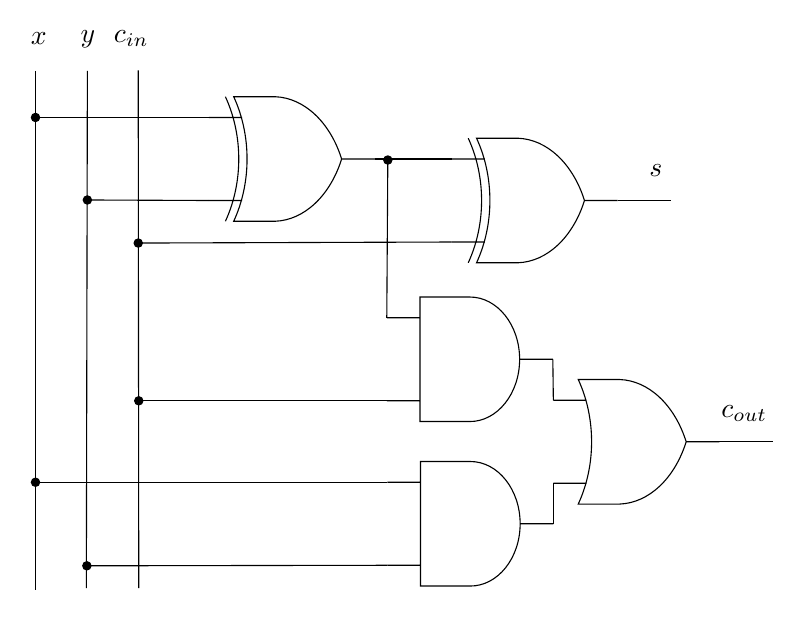
\begin{tikzpicture}[x=0.75pt,y=0.75pt,yscale=-1,xscale=1]\centering
		%uncomment if require: \path (0,625); %set diagram left start at 0, and has height of 625
		
		%Shape: Xor Gate [id:dp22227458736036843] 
		\draw   (146,63) -- (166,63) .. controls (179.95,63.54) and (192.42,75.23) .. (198,93) .. controls (192.42,110.77) and (179.95,122.46) .. (166,123) -- (146,123) .. controls (154.57,104.44) and (154.57,81.56) .. (146,63) -- cycle (134,73) -- (150,73) (134,113) -- (150,113) (198,93) -- (214,93) (142,63) .. controls (150.57,81.56) and (150.57,104.44) .. (142,123) ;
		%Shape: Xor Gate [id:dp9558597305912817] 
		\draw   (263,83) -- (283,83) .. controls (296.95,83.54) and (309.42,95.23) .. (315,113) .. controls (309.42,130.77) and (296.95,142.46) .. (283,143) -- (263,143) .. controls (271.57,124.44) and (271.57,101.56) .. (263,83) -- cycle (251,93) -- (267,93) (251,133) -- (267,133) (315,113) -- (331,113) (259,83) .. controls (267.57,101.56) and (267.57,124.44) .. (259,143) ;
		%Straight Lines [id:da3073236030985753] 
		\draw    (50.5,50.5) -- (50.5,300.5) ;
		%Straight Lines [id:da3888123726899575] 
		\draw    (75.5,50.5) -- (75,299.75) ;
		%Straight Lines [id:da35097176458483736] 
		\draw    (100,50.25) -- (100.25,299.75) ;
		%Straight Lines [id:da5953784724922828] 
		\draw    (214,93) -- (251,93) ;
		%Straight Lines [id:da3222355089037585] 
		\draw    (50.5,73) -- (134,73) ;
		%Shape: Circle [id:dp2883615095456349] 
		\draw  [fill={rgb, 255:red, 0; green, 0; blue, 0 }  ,fill opacity=1 ] (52.5,73) .. controls (52.5,71.9) and (51.6,71) .. (50.5,71) .. controls (49.4,71) and (48.5,71.9) .. (48.5,73) .. controls (48.5,74.1) and (49.4,75) .. (50.5,75) .. controls (51.6,75) and (52.5,74.1) .. (52.5,73) -- cycle ;
		%Straight Lines [id:da5899065332833413] 
		\draw    (75.5,112.75) -- (134,113) ;
		%Shape: Circle [id:dp6016016248611964] 
		\draw  [fill={rgb, 255:red, 0; green, 0; blue, 0 }  ,fill opacity=1 ] (77.5,112.75) .. controls (77.5,111.65) and (76.6,110.75) .. (75.5,110.75) .. controls (74.4,110.75) and (73.5,111.65) .. (73.5,112.75) .. controls (73.5,113.85) and (74.4,114.75) .. (75.5,114.75) .. controls (76.6,114.75) and (77.5,113.85) .. (77.5,112.75) -- cycle ;
		%Straight Lines [id:da24994922912424933] 
		\draw    (100,133.5) -- (251,133) ;
		%Shape: Circle [id:dp7950607903721081] 
		\draw  [fill={rgb, 255:red, 0; green, 0; blue, 0 }  ,fill opacity=1 ] (102,133.5) .. controls (102,132.4) and (101.1,131.5) .. (100,131.5) .. controls (98.9,131.5) and (98,132.4) .. (98,133.5) .. controls (98,134.6) and (98.9,135.5) .. (100,135.5) .. controls (101.1,135.5) and (102,134.6) .. (102,133.5) -- cycle ;
		%Straight Lines [id:da5076937403756383] 
		\draw    (331,113) -- (356.75,113) ;
		%Shape: And Gate [id:dp8071044679947741] 
		\draw   (235.75,159.5) -- (259.75,159.5) .. controls (273,159.5) and (283.75,172.94) .. (283.75,189.5) .. controls (283.75,206.06) and (273,219.5) .. (259.75,219.5) -- (235.75,219.5) -- (235.75,159.5) -- cycle (219.75,169.5) -- (235.75,169.5) (219.75,209.5) -- (235.75,209.5) (283.75,189.5) -- (299.75,189.5) ;
		%Straight Lines [id:da3876484716368205] 
		\draw    (219.75,169.5) -- (220.25,92.5) ;
		%Shape: Circle [id:dp7628595620557719] 
		\draw  [fill={rgb, 255:red, 0; green, 0; blue, 0 }  ,fill opacity=1 ] (222.25,93.5) .. controls (222.25,92.4) and (221.35,91.5) .. (220.25,91.5) .. controls (219.15,91.5) and (218.25,92.4) .. (218.25,93.5) .. controls (218.25,94.6) and (219.15,95.5) .. (220.25,95.5) .. controls (221.35,95.5) and (222.25,94.6) .. (222.25,93.5) -- cycle ;
		%Straight Lines [id:da1914868824551612] 
		\draw    (219.75,209.5) -- (100.25,209.5) ;
		%Shape: Circle [id:dp08491219949794826] 
		\draw  [fill={rgb, 255:red, 0; green, 0; blue, 0 }  ,fill opacity=1 ] (102.25,209.5) .. controls (102.25,208.4) and (101.35,207.5) .. (100.25,207.5) .. controls (99.15,207.5) and (98.25,208.4) .. (98.25,209.5) .. controls (98.25,210.6) and (99.15,211.5) .. (100.25,211.5) .. controls (101.35,211.5) and (102.25,210.6) .. (102.25,209.5) -- cycle ;
		%Shape: And Gate [id:dp40156934307935765] 
		\draw   (236,238.75) -- (260,238.75) .. controls (273.25,238.75) and (284,252.19) .. (284,268.75) .. controls (284,285.31) and (273.25,298.75) .. (260,298.75) -- (236,298.75) -- (236,238.75) -- cycle (220,248.75) -- (236,248.75) (220,288.75) -- (236,288.75) (284,268.75) -- (300,268.75) ;
		%Straight Lines [id:da8360513967661218] 
		\draw    (220,248.75) -- (50.5,248.75) ;
		%Straight Lines [id:da35301927256757804] 
		\draw    (75.25,289) -- (220,288.75) ;
		%Shape: Circle [id:dp8426807814067807] 
		\draw  [fill={rgb, 255:red, 0; green, 0; blue, 0 }  ,fill opacity=1 ] (52.5,248.75) .. controls (52.5,247.65) and (51.6,246.75) .. (50.5,246.75) .. controls (49.4,246.75) and (48.5,247.65) .. (48.5,248.75) .. controls (48.5,249.85) and (49.4,250.75) .. (50.5,250.75) .. controls (51.6,250.75) and (52.5,249.85) .. (52.5,248.75) -- cycle ;
		%Shape: Circle [id:dp918579776520918] 
		\draw  [fill={rgb, 255:red, 0; green, 0; blue, 0 }  ,fill opacity=1 ] (77.25,289) .. controls (77.25,287.9) and (76.35,287) .. (75.25,287) .. controls (74.15,287) and (73.25,287.9) .. (73.25,289) .. controls (73.25,290.1) and (74.15,291) .. (75.25,291) .. controls (76.35,291) and (77.25,290.1) .. (77.25,289) -- cycle ;
		%Shape: Or Gate [id:dp015181351581308844] 
		\draw   (312,199.25) -- (332,199.25) .. controls (345.95,199.79) and (358.42,211.48) .. (364,229.25) .. controls (358.42,247.02) and (345.95,258.71) .. (332,259.25) -- (312,259.25) .. controls (320.57,240.69) and (320.57,217.81) .. (312,199.25) -- cycle (300,209.25) -- (316,209.25) (300,249.25) -- (316,249.25) (364,229.25) -- (380,229.25) ;
		%Straight Lines [id:da12371997688817848] 
		\draw    (299.75,189.5) -- (300,209.25) ;
		%Straight Lines [id:da7226790821082669] 
		\draw    (300,249.25) -- (300,268.75) ;
		%Straight Lines [id:da35453108229640606] 
		\draw    (380,229.25) -- (405.75,229.25) ;
		
		% Text Node
		\draw (47,31) node [anchor=north west][inner sep=0.75pt]   [align=left] {$x$};
		% Text Node
		\draw (71,30) node [anchor=north west][inner sep=0.75pt]   [align=left] {$y$};
		% Text Node
		\draw (87,30) node [anchor=north west][inner sep=0.75pt]   [align=left] {$c_{in}$};
		% Text Node
		\draw (345,94.25) node [anchor=north west][inner sep=0.75pt]   [align=left] {$s$};
		% Text Node
		\draw (379.75,210.5) node [anchor=north west][inner sep=0.75pt]   [align=left] {$c_{out}$};
	\end{tikzpicture}\bigbreak
\end{center}

From now on, we can write this as a black box as follows

\begin{center}
	\begin{tikzpicture}[
		fulladder/.style={draw, minimum size=3cm,
			label={[anchor=west]left:$c_\text{out}$},
			label={[anchor=south]below:$s$},
			label={[anchor=east]right:$c_\text{in}$},
			label={[anchor=north]65:$y$},
			label={[anchor=north]115:$x\vphantom{y}$},
			label={[anchor=center]center:F-A}
		}]
		
		\node[fulladder] (a) {};
		
		\draw[<-] (a.115) --++(90:0.5cm) node [above] {};
		\draw[<-] (a.65) --++(90:0.5cm) node [above] {};
		\draw[<-] (a.east) --++(0:0.5cm) node [right] {};
		\draw[->] (a.west) --++(180:0.5cm) node [left] {};
		\draw[->] (a.south) --++(-90:0.5cm) node [below] {};
	\end{tikzpicture}
\end{center}\bigbreak


\subsubsection{8 bit Binary Adder}
\bigbreak

We would like to add two numbers expressed each in 8 bits.\\

\begin{center}
	\begin{tabular}{ccccc}
		& \tiny & \tiny & \tiny & \tiny \\
		& $x_{7}$ & ... & $x_{1}$ & $x_{0}$ \\
		+ & $y_{7}$ & ... & $y_{1}$ & $y_{0}$ \\
		\hline
		$c_{out}$ & $s_{7}$ & ... & $s_{1}$ & $s_{0}$ \\\smallskip
	\end{tabular}
\end{center}\bigbreak

The number of inputs is 16 and the number of outputs is 9. This program has $2^16 \approx 64000$ combinations... Quite the truth table. We will skip that step.\\

Instead we will construct the logic diagram by chaining full adders.\\

\centerline{
	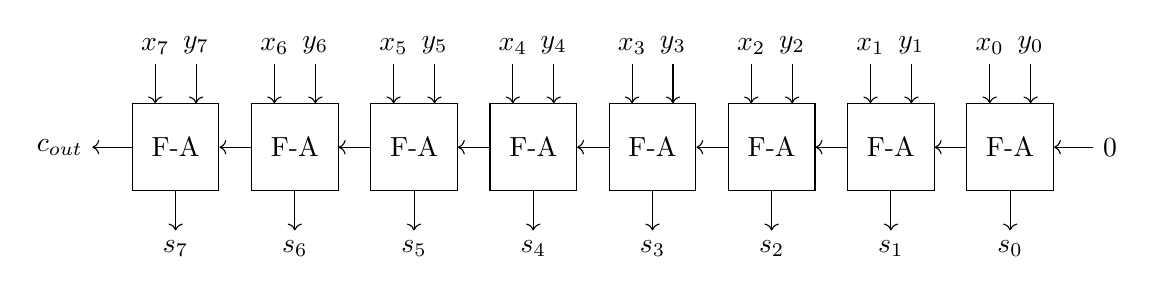
\begin{tikzpicture}[
		fulladder/.style={draw, minimum size=1.1cm,
			label={[anchor=center]center:F-A}
		}]
		
		\node[fulladder] (faL) {};
		\node[fulladder, right=0.4cm of faL] (fam2) {};
		\node[fulladder, right=0.4cm of fam2] (fam3) {};
		\node[fulladder, right=0.4cm of fam3] (fam4) {};
		\node[fulladder, right=0.4cm of fam4] (fam5) {};
		\node[fulladder, right=0.4cm of fam5] (fam6) {};
		\node[fulladder, right=0.4cm of fam6] (fam7) {};
		\node[fulladder, right=0.4cm of fam7] (faR) {};
		
		\draw[<-] (faL.115) --++(90:0.5cm) node [above] {$x_7$};
		\draw[<-] (faL.65) --++(90:0.5cm) node [above] {$y_7$};
		\draw[->] (faL.south) --++(-90:0.5cm) node [below] {$s_7$};
		\draw[<-] (faL.east) -- (fam2.west);
		\draw[->] (faL.west) --++(180:0.5cm) node [left] {$c_{out}$};
		
		\draw[<-] (fam2.115) --++(90:0.5cm) node [above] {$x_6$};
		\draw[<-] (fam2.65) --++(90:0.5cm) node [above] {$y_6$};
		\draw[->] (fam2.south) --++(-90:0.5cm) node [below] {$s_6$};
		\draw[<-] (fam2.east) -- (fam3.west);
		
		\draw[<-] (fam3.115) --++(90:0.5cm) node [above] {$x_5$};
		\draw[<-] (fam3.65) --++(90:0.5cm) node [above] {$y_5$};
		\draw[->] (fam3.south) --++(-90:0.5cm) node [below] {$s_5$};
		\draw[<-] (fam3.east) -- (fam4.west);
		
		\draw[<-] (fam4.115) --++(90:0.5cm) node [above] {$x_4$};
		\draw[<-] (fam4.65) --++(90:0.5cm) node [above] {$y_4$};
		\draw[->] (fam4.south) --++(-90:0.5cm) node [below] {$s_4$};
		\draw[<-] (fam4.east) -- (fam5.west);
		
		\draw[<-] (fam5.115) --++(90:0.5cm) node [above] {$x_3$};
		\draw[<-] (fam5.65) --++(90:0.5cm) node [above] {$y_3$};
		\draw[->] (fam5.south) --++(-90:0.5cm) node [below] {$s_3$};
		\draw[<-] (fam5.east) -- (fam6.west);
		
		\draw[<-] (fam6.115) --++(90:0.5cm) node [above] {$x_2$};
		\draw[<-] (fam6.65) --++(90:0.5cm) node [above] {$y_2$};
		\draw[->] (fam6.south) --++(-90:0.5cm) node [below] {$s_2$};
		\draw[<-] (fam6.east) -- (fam7.west);
		
		\draw[<-] (fam7.115) --++(90:0.5cm) node [above] {$x_1$};
		\draw[<-] (fam7.65) --++(90:0.5cm) node [above] {$y_1$};
		\draw[->] (fam7.south) --++(-90:0.5cm) node [below] {$s_1$};
		\draw[<-] (fam7.east) -- (faR.west);
		
		\draw[<-] (faR.115) --++(90:0.5cm) node [above] {$x_0$};
		\draw[<-] (faR.65) --++(90:0.5cm) node [above] {$y_0$};
		\draw[->] (faR.south) --++(-90:0.5cm) node [below] {$s_0$};
		\draw[<-] (faR.east) --++(0:0.5cm) node [right] {$0$};
	\end{tikzpicture}
}\bigbreak

We can compact the \textbf{8 bit adder} in a black box as follows.\\

\begin{center}
	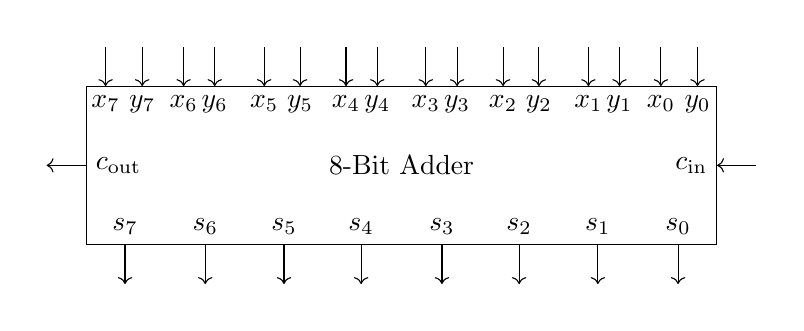
\begin{tikzpicture}[
		adder8bit/.style={draw, minimum width=8cm, minimum height=2cm,
			label={[anchor=west]left:$c_\text{out}$},
			label={[anchor=east]right:$c_\text{in}$},
			label={[anchor=south]344:$s_0$},
			label={[anchor=south]338:$s_1$},
			label={[anchor=south]326:$s_2$},
			label={[anchor=south]297:$s_3$},
			label={[anchor=south]243:$s_4$},
			label={[anchor=south]214:$s_5$},
			label={[anchor=south]202:$s_6$},
			label={[anchor=south]196:$s_7$},
			label={[anchor=north]17:$x_0$},
			label={[anchor=north]23:$x_1$},
			label={[anchor=north]38:$x_2$},
			label={[anchor=north]73:$x_3$},
			label={[anchor=north]125:$x_4$},
			label={[anchor=north]150:$x_5$},
			label={[anchor=north]160:$x_6$},
			label={[anchor=north]165:$x_7$},
			label={[anchor=north]15:$y_0$},
			label={[anchor=north]20:$y_1$},
			label={[anchor=north]30:$y_2$},
			label={[anchor=north]55:$y_3$},
			label={[anchor=north]107:$y_4$},
			label={[anchor=north]142:$y_5$},
			label={[anchor=north]157:$y_6$},
			label={[anchor=north]163:$y_7$},
			label={[anchor=center]center:8-Bit Adder}
		}]
		
		\node[adder8bit] (a8b) {};
		
		%outputs
		\draw[->] (a8b.344) --++(90:-0.5cm) node [below] {};
		\draw[->] (a8b.338) --++(90:-0.5cm) node [below] {};
		\draw[->] (a8b.326) --++(90:-0.5cm) node [below] {};
		\draw[->] (a8b.297) --++(90:-0.5cm) node [below] {};
		\draw[->] (a8b.243) --++(90:-0.5cm) node [below] {};
		\draw[->] (a8b.214) --++(90:-0.5cm) node [below] {};
		\draw[->] (a8b.202) --++(90:-0.5cm) node [below] {};
		\draw[->] (a8b.196) --++(90:-0.5cm) node [below] {};
		
		%inputs
		%xs
		\draw[<-] (a8b.17) --++(90:0.5cm) node [above] {};
		\draw[<-] (a8b.23) --++(90:0.5cm) node [above] {};
		\draw[<-] (a8b.38) --++(90:0.5cm) node [above] {};
		\draw[<-] (a8b.73) --++(90:0.5cm) node [above] {};
		\draw[<-] (a8b.125) --++(90:0.5cm) node [above] {};
		\draw[<-] (a8b.150) --++(90:0.5cm) node [above] {};
		\draw[<-] (a8b.160) --++(90:0.5cm) node [above] {};
		\draw[<-] (a8b.165) --++(90:0.5cm) node [above] {};
		%ys
		\draw[<-] (a8b.15) --++(90:0.5cm) node [above] {};
		\draw[<-] (a8b.20) --++(90:0.5cm) node [above] {};
		\draw[<-] (a8b.30) --++(90:0.5cm) node [above] {};
		\draw[<-] (a8b.55) --++(90:0.5cm) node [above] {};
		\draw[<-] (a8b.107) --++(90:0.5cm) node [above] {};
		\draw[<-] (a8b.142) --++(90:0.5cm) node [above] {};
		\draw[<-] (a8b.157) --++(90:0.5cm) node [above] {};
		\draw[<-] (a8b.163) --++(90:0.5cm) node [above] {};
		
		% carry in/out
		\draw[<-] (a8b.east) --++(0:0.5cm) node [right] {};
		\draw[->] (a8b.west) --++(180:0.5cm) node [left] {};
	\end{tikzpicture}
\end{center}\bigbreak

Let us now see if we can make an \textbf{8-bit subtractor} now. We want to find $x-y = x + \text{2's complement of }y = x + \bar{y} + 1$. Therefore, all we have to do to make a subtractor is to invert $y_i$ and set $c_{in} = 1$. The following is the diagram.\\

\begin{center}
	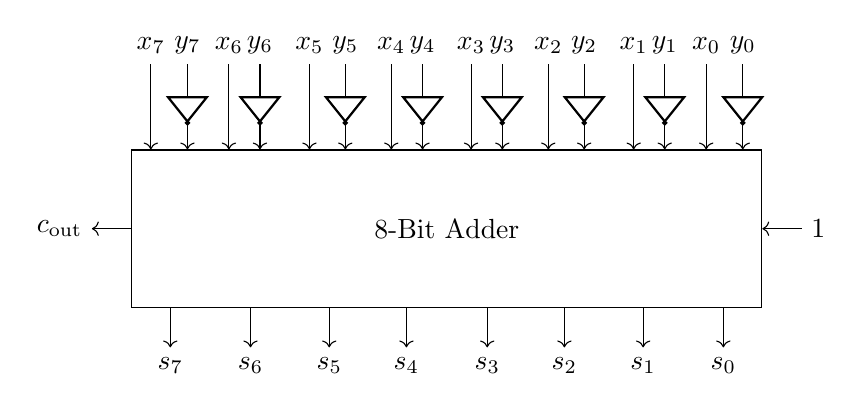
\begin{tikzpicture}[
		adder8bit/.style={draw, minimum width=8cm, minimum height=2cm,
			label={[anchor=center]center:8-Bit Adder}
		}]
		
		\node[adder8bit] (a8b) {};
		
		\node at (a8b.15)[not port, rotate=-90, scale=0.35, xshift=-1.4cm](noty0){};
		\node at (a8b.20)[not port, rotate=-90, scale=0.35, xshift=-1.4cm](noty1){};
		\node at (a8b.30)[not port, rotate=-90, scale=0.35, xshift=-1.4cm](noty2){};
		\node at (a8b.55)[not port, rotate=-90, scale=0.35, xshift=-1.4cm](noty3){};
		\node at (a8b.107)[not port, rotate=-90, scale=0.35, xshift=-1.4cm](noty4){};
		\node at (a8b.142)[not port, rotate=-90, scale=0.35, xshift=-1.4cm](noty5){};
		\node at (a8b.157)[not port, rotate=-90, scale=0.35, xshift=-1.4cm](noty6){};
		\node at (a8b.163)[not port, rotate=-90, scale=0.35, xshift=-1.4cm](noty7){};
		
		%outputs
		\draw[->] (a8b.344) --++(90:-0.5cm) node [below] {$s_0$};
		\draw[->] (a8b.338) --++(90:-0.5cm) node [below] {$s_1$};
		\draw[->] (a8b.326) --++(90:-0.5cm) node [below] {$s_2$};
		\draw[->] (a8b.297) --++(90:-0.5cm) node [below] {$s_3$};
		\draw[->] (a8b.243) --++(90:-0.5cm) node [below] {$s_4$};
		\draw[->] (a8b.214) --++(90:-0.5cm) node [below] {$s_5$};
		\draw[->] (a8b.202) --++(90:-0.5cm) node [below] {$s_6$};
		\draw[->] (a8b.196) --++(90:-0.5cm) node [below] {$s_7$};
		
		%inputs
		%xs
		\draw[<-] (a8b.17) --++(90:1.09cm) node [above] {$x_0$};
		\draw[<-] (a8b.23) --++(90:1.09cm) node [above] {$x_1$};
		\draw[<-] (a8b.38) --++(90:1.09cm) node [above] {$x_2$};
		\draw[<-] (a8b.73) --++(90:1.09cm) node [above] {$x_3$};
		\draw[<-] (a8b.125) --++(90:1.09cm) node [above] {$x_4$};
		\draw[<-] (a8b.150) --++(90:1.09cm) node [above] {$x_5$};
		\draw[<-] (a8b.160) --++(90:1.09cm) node [above] {$x_6$};
		\draw[<-] (a8b.165) --++(90:1.09cm) node [above] {$x_7$};
		
		%ys
		\draw (noty0.in)--++(90:0.35cm) node[above]{$y_0$};
		\draw (noty1.in)--++(90:0.35cm) node[above]{$y_1$};
		\draw (noty2.in)--++(90:0.35cm) node[above]{$y_2$};
		\draw (noty3.in)--++(90:0.35cm) node[above]{$y_3$};
		\draw (noty4.in)--++(90:0.35cm) node[above]{$y_4$};
		\draw (noty5.in)--++(90:0.35cm) node[above]{$y_5$};
		\draw (noty6.in)--++(90:0.35cm) node[above]{$y_6$};
		\draw (noty7.in)--++(90:0.35cm) node[above]{$y_7$};
		
		\draw[<-] (a8b.15) -- (noty0.out);
		\draw[<-] (a8b.20) -- (noty1.out);
		\draw[<-] (a8b.30) -- (noty2.out);
		\draw[<-] (a8b.55) -- (noty3.out);
		\draw[<-] (a8b.107) -- (noty4.out);
		\draw[<-] (a8b.142) -- (noty5.out);
		\draw[<-] (a8b.157) -- (noty6.out);
		\draw[<-] (a8b.163) -- (noty7.out);
		
		% carry in/out
		\draw[<-] (a8b.east) --++(0:0.5cm) node [right] {$1$};
		\draw[->] (a8b.west) --++(180:0.5cm) node [left] {$c_\text{out}$};
	\end{tikzpicture}
\end{center}\bigbreak\bigbreak\bigbreak


\subsubsection{8-Bit Adder/Subtractor}
\bigbreak

We now want to make a circuit that take $x$ and $y$ (which are 8 bit integers), and computes $x+y$ or $x-y$ based on a selection made by the user. We can do this using XOR gates. \\

\begin{center}
	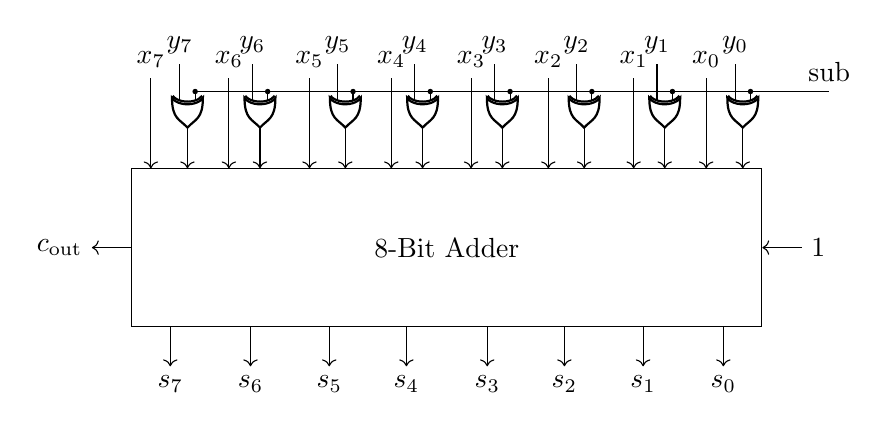
\begin{tikzpicture}[
		adder8bit/.style={draw, minimum width=8cm, minimum height=2cm,
			label={[anchor=center]center:8-Bit Adder}
		}]
		
		\node[adder8bit] (a8b) {};
		
		\node at (a8b.15)[xor port, rotate=-90, scale=0.35, xshift=-1.4cm](xory0){};
		\node at (a8b.20)[xor port, rotate=-90, scale=0.35, xshift=-1.4cm](xory1){};
		\node at (a8b.30)[xor port, rotate=-90, scale=0.35, xshift=-1.4cm](xory2){};
		\node at (a8b.55)[xor port, rotate=-90, scale=0.35, xshift=-1.4cm](xory3){};
		\node at (a8b.107)[xor port, rotate=-90, scale=0.35, xshift=-1.4cm](xory4){};
		\node at (a8b.142)[xor port, rotate=-90, scale=0.35, xshift=-1.4cm](xory5){};
		\node at (a8b.157)[xor port, rotate=-90, scale=0.35, xshift=-1.4cm](xory6){};
		\node at (a8b.163)[xor port, rotate=-90, scale=0.35, xshift=-1.4cm](xory7){};
		
		%outputs
		\draw[->] (a8b.344) --++(90:-0.5cm) node [below] {$s_0$};
		\draw[->] (a8b.338) --++(90:-0.5cm) node [below] {$s_1$};
		\draw[->] (a8b.326) --++(90:-0.5cm) node [below] {$s_2$};
		\draw[->] (a8b.297) --++(90:-0.5cm) node [below] {$s_3$};
		\draw[->] (a8b.243) --++(90:-0.5cm) node [below] {$s_4$};
		\draw[->] (a8b.214) --++(90:-0.5cm) node [below] {$s_5$};
		\draw[->] (a8b.202) --++(90:-0.5cm) node [below] {$s_6$};
		\draw[->] (a8b.196) --++(90:-0.5cm) node [below] {$s_7$};
		
		%inputs
		%xs
		\draw[<-] (a8b.17) --++(90:1.15cm) node [above] {$x_0$};
		\draw[<-] (a8b.23) --++(90:1.15cm) node [above] {$x_1$};
		\draw[<-] (a8b.38) --++(90:1.15cm) node [above] {$x_2$};
		\draw[<-] (a8b.73) --++(90:1.15cm) node [above] {$x_3$};
		\draw[<-] (a8b.125) --++(90:1.15cm) node [above] {$x_4$};
		\draw[<-] (a8b.150) --++(90:1.15cm) node [above] {$x_5$};
		\draw[<-] (a8b.160) --++(90:1.15cm) node [above] {$x_6$};
		\draw[<-] (a8b.165) --++(90:1.15cm) node [above] {$x_7$};
		
		%ys
		\draw (xory0.in 2)--++(90:0.35cm) node[above]{$y_0$};
		\draw (xory1.in 2)--++(90:0.35cm) node[above]{$y_1$};
		\draw (xory2.in 2)--++(90:0.35cm) node[above]{$y_2$};
		\draw (xory3.in 2)--++(90:0.35cm) node[above]{$y_3$};
		\draw (xory4.in 2)--++(90:0.35cm) node[above]{$y_4$};
		\draw (xory5.in 2)--++(90:0.35cm) node[above]{$y_5$};
		\draw (xory6.in 2)--++(90:0.35cm) node[above]{$y_6$};
		\draw (xory7.in 2)--++(90:0.35cm) node[above]{$y_7$};
		
		\draw[<-] (a8b.15) -- (xory0.out);
		\draw[<-] (a8b.20) -- (xory1.out);
		\draw[<-] (a8b.30) -- (xory2.out);
		\draw[<-] (a8b.55) -- (xory3.out);
		\draw[<-] (a8b.107) -- (xory4.out);
		\draw[<-] (a8b.142) -- (xory5.out);
		\draw[<-] (a8b.157) -- (xory6.out);
		\draw[<-] (a8b.163) -- (xory7.out);
		
		\draw (xory7.in 1) node [circle,fill,inner sep=0.7pt]{} -- (xory6.in 1) node [circle,fill,inner sep=0.7pt]{} -- (xory5.in 1) node [circle,fill,inner sep=0.7pt]{} -- (xory4.in 1) node [circle,fill,inner sep=0.7pt]{} -- (xory3.in 1) node [circle,fill,inner sep=0.7pt]{} -- (xory2.in 1) node [circle,fill,inner sep=0.7pt]{} -- (xory1.in 1) node [circle,fill,inner sep=0.7pt]{} -- (xory0.in 1) node [circle,fill,inner sep=0.7pt]{} -- ++(1cm, 0) node[above]{sub};
		
		% carry in/out
		\draw[<-] (a8b.east) --++(0:0.5cm) node [right] {$1$};
		\draw[->] (a8b.west) --++(180:0.5cm) node [left] {$c_\text{out}$};
	\end{tikzpicture}
\end{center}\bigbreak


\subsubsection{Moving Forward}
\bigbreak

So far we have used the sum of products method to find

\begin{itemize}
	\item Arthmetic circuits (Adder \& Subtractor)
	\item Logic circuits (Equality test)
\end{itemize}\bigbreak

Both of these types of circuits together are part of the \textbf{Arithmetic Logic Unit} (ALU).\\

The \textit{CPU} is made of the \textit{ALU} and the \textit{Control Unit} (CU). The control unit is responsible for managing the ALU and memory. The control unit is composed of combinational circuits. These circuits perform control operations. What are these?

\begin{itemize}
	\item Selection: Select data from memory
	\item Decoding: Decode the operation code
	\item Encoding
	\item ...
\end{itemize}\bigbreak

We will know build control circuits for Selection and Decoding.\\


\subsubsection{The Multiplexer}
\bigbreak

The \textbf{multiplexer} is a selection circuit which

\begin{itemize}
	\item selects one of many inputs
	\item direct it to the output
\end{itemize}\bigbreak

A multiplexer is denoted as MUX. A MUX has

\begin{itemize}
	\item $2^n$ inputs: $I_0$, $I_1$, $I_2$, ..., $I_{2^n-1}$ where $I_i \in \{0, 1\}$
	\item 1 output
	\item $n$ selection lines: $s_0$, $s_1$, ..., $s_{n-1}$
\end{itemize}\bigbreak

The decimal value of $s = s_{n-1} ... s_1s_0$ is the \textit{index of the input that will be directed to the output}. The multiplexer diagram is\\

\begin{center}
	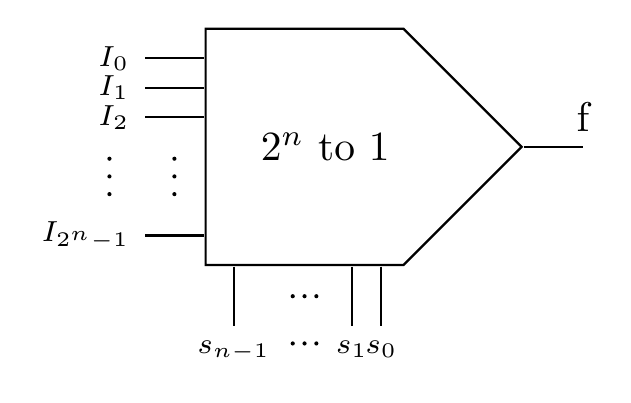
\begin{tikzpicture}[multiplexer/.style={
			draw,
			signal,
			shape border uses incircle, 
			shape border rotate=270,
			minimum width=2.5cm, 
			minimum height=2cm,
		}, thick,scale=1.5,every node/.style={transform shape}]
		\node[multiplexer] (mul) at (0,0) {~~~$2^n$ to 1};
		\draw (mul.east) --++(0.5cm,0) node[above]{f};
		
		\draw (mul.west)++(0, 0.75cm) --++(-0.5cm,0) node[left]{\scriptsize $I_0$};
		\draw (mul.west)++(0, 0.50cm) --++(-0.5cm,0) node[left]{\scriptsize $I_1$};
		\draw (mul.west)++(0, 0.25cm) --++(-0.5cm,0) node[left]{\scriptsize $I_2$};
		\draw (mul.west)++(-0.25cm, -0.1cm) node[circle, fill, inner sep=0.02]{} ++(-0.55cm, 0) node[circle, fill, inner sep=0.02]{};
		\draw (mul.west)++(-0.25cm, -0.25cm) node[circle, fill, inner sep=0.02]{} ++(-0.55cm, 0) node[circle, fill, inner sep=0.02]{};
		\draw (mul.west)++(-0.25cm, -0.4cm) node[circle, fill, inner sep=0.02]{} ++(-0.55cm, 0) node[circle, fill, inner sep=0.02]{};
		\draw (mul.west)++(0, -0.75cm) --++(-0.5cm,0) node[left]{\scriptsize $I_{2^n-1}$};
		
		\draw (mul.south)++(-0.6cm, 0) --++(0, -0.5cm) node[below]{\scriptsize $s_{n-1}$};
		\draw (mul.south)++(0.4cm, 0) --++(0, -0.5cm) node[below]{\scriptsize $s_{1}$};
		\draw (mul.south)++(0.1cm, -0.25cm) node[circle, fill, inner sep=0.02]{} ++(0, -0.4cm) node[circle, fill, inner sep=0.02]{};
		\draw (mul.south)++(0.0cm, -0.25cm) node[circle, fill, inner sep=0.02]{} ++(0, -0.4cm) node[circle, fill, inner sep=0.02]{};
		\draw (mul.south)++(-0.1cm, -0.25cm) node[circle, fill, inner sep=0.02]{} ++(0, -0.4cm) node[circle, fill, inner sep=0.02]{};
		\draw (mul.south)++(0.65cm, 0) --++(0, -0.5cm) node[below]{\scriptsize $s_{0}$};
	\end{tikzpicture}
\end{center}\bigbreak

If $s_{n-1} ... s_1s_0 = (00...0)_2 = (0)_{10} \implies f = I_0$.\\
If $s_{n-1} ... s_1s_0  = (00...1)_2 = (1)_{10} \implies f = I_1$. And so on...\\
If $s_{n-1} ... s_1s_0  = (11...1)_2 = (2^n-1)_{10} \implies f = I_{2^n-1}$.\\

An everyday example of a multiplexer is the decimal multiplexer on a remote control for a TV. If you have $100 = 10^2$ channels (0 to 99), in order to select one, you choose two decimal numbers (say 8 and 5) to be your $s_1$ and $s_0$. The multiplexer then connects the input (in this case channel 85) to the output (TV). \\
\pagebreak


\subsubsection{2 to 1 Multiplexer}
\bigbreak

A 2 to 1 multiplexer will have $n=1$ and therefore $2^n-1 = 2^1-1 = 2$ inputs ($I_0$ and $I_1$) with $n=1$ selection lines ($s_0 \equiv s$) and an output $f$. The corresponding diagram is\\

\begin{center}
	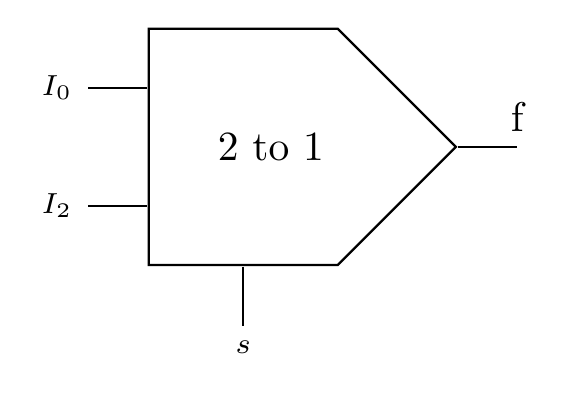
\begin{tikzpicture}[multiplexer/.style={
			draw,
			signal,
			shape border uses incircle, 
			shape border rotate=270,
			minimum width=2.5cm, 
			minimum height=2cm,
		}, thick,scale=1.5,every node/.style={transform shape}]
		\node[multiplexer] (mul) at (0,0) {~~~~2 to 1};
		\draw (mul.east) --++(0.5cm,0) node[above]{f};
		
		\draw (mul.west)++(0, 0.5cm) --++(-0.5cm,0) node[left]{\scriptsize $I_0$};
		\draw (mul.west)++(0, -0.5cm) --++(-0.5cm,0) node[left]{\scriptsize $I_{2}$};
		
		\draw (mul.south) --++(0, -0.5cm) node[below]{\scriptsize $s$};
	\end{tikzpicture}
\end{center}\bigbreak

If $s=0$ then $f=I_0$ and if $s=1$ then $f=I_1$. We will now use the \textit{sum of products} technique (as usual). The truth table of the 2 to 1 multiplexer is\bigbreak

\begin{center}
	\begin{tabular}{|c|c||c|c|}
		$I_1$ & $I_0$ & $s$ & $f$ 	\\\hline
		   0  &   0   &  0  &  0  	\\
		   0  &   0   &  1  &  0  	\\
		   0  &   1   &  0  &  1  	\\
		   0  &   1   &  1  &  0  	\\
		   1  &   0   &  0  &  0  	\\
		   1  &   0   &  1  &  1  	\\
		   1  &   1   &  0  &  1  	\\
		   1  &   1   &  1  &  1  	\\
	\end{tabular}
	\bigbreak
\end{center}

The Boolean expression is therefore $f = \bar{I_1}I_0\bar{s} + I_1\bar{I_0}s + I_1I_0\bar{s} + I_1I_0s$. We can simply this expression.

\begin{align*}
	f &= \bar{I_1}I_0\bar{s} + I_1\bar{I_0}s + I_1I_0\bar{s} + I_1I_0s\\
	  &= I_0\bar{s}(\bar{I_1} + I_1) + I_1s(\bar{I_0} + I_0)\\
	  &= I_0\bar{s} + I_1s
\end{align*}\bigbreak

Thus, $f=I_0\bar{s} + I_1s$. We can draw this diagram as\bigbreak


\begin{center}
	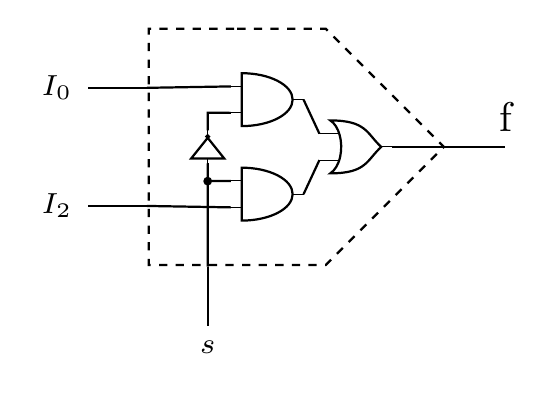
\begin{tikzpicture}[multiplexer/.style={
			draw,
			signal,
			shape border uses incircle, 
			shape border rotate=270,
			minimum width=2.5cm, 
			minimum height=2cm,
			dashed
		}, thick,scale=1.5,every node/.style={transform shape}]
		\node[multiplexer] (mul) at (0,0) {};
		\draw (mul.east) --++(0.5cm,0) node[above]{f};
		
		\draw (mul.west)++(0, 0.5cm) --++(-0.5cm,0) node[left]{\scriptsize $I_0$};
		\draw (mul.west)++(0, -0.5cm) --++(-0.5cm,0) node[left]{\scriptsize $I_{2}$};
		
		\draw (mul.south)++(-0.25cm, 0) --++(0, -0.5cm) node[below]{\scriptsize $s$};
		
		\node at (-0.25cm, 0)[not port, rotate=90, scale=0.2, thin](mynot){};
		\node at (0.5cm, 0.4cm)[and port, scale=0.4, thin](upperand){};
		\node at (0.5cm, -0.4cm)[and port, scale=0.4, thin](lowerand){};
		\node at (1.25cm, 0)[or port, scale=0.4, thin](myor){};
		
		\draw (mul.west)++(0, 0.5cm) -- (upperand.in 1);
		\draw (mul.west)++(0, -0.5cm) -- (lowerand.in 2);
		\draw (upperand.out) -- (myor.in 1);
		\draw (lowerand.out) -- (myor.in 2);
		\draw (myor.out) -- (mul.east);
		\draw (mynot.out) -- ++ (0, 0.15cm) --(upperand.in 2);
		\draw (mul.south)++(-0.25cm, 0) -- (mynot.in) ++ (0, -0.15cm) node[circle, fill, inner sep=0.75]{} --(lowerand.in 1);
		\draw (mynot.in) ++ (0, -0.15cm) -- (mynot.in);
	\end{tikzpicture}
\end{center}\bigbreak

In order to scale this up to larger multiplexers, we need a different method because the standard sum of products method is too inefficient.\\

To do this, we will make a compactified truth table by only using s as an input and instead consider them as the values of the output.\\

\begin{center}
	\begin{tabular}{|c||c|}
		$s$ & $f$\\\hline
		0  &   $I_0$\\
		1  &   $I_1$\\
	\end{tabular}
	\bigbreak
\end{center}

Now we can get a Boolean expression from this truth table now. Using this method, we and each of the outputs of $f$ (in this case $I_0$ and $I_1$) with the inputs (following the same rule as before, where a not in inserted if the value is 0). Namely, here we get that $f = I_0\bar{s} + I_1s$. Note that this is the same as the expression we got using the previous method, but with less steps.\\


\subsubsection{4 to 1 Multiplexer}
\bigbreak

In a 4 to 1 multiplexer, we will have 4 inputs and 2 selection lines. The multiplexer looks like\\

\begin{center}
	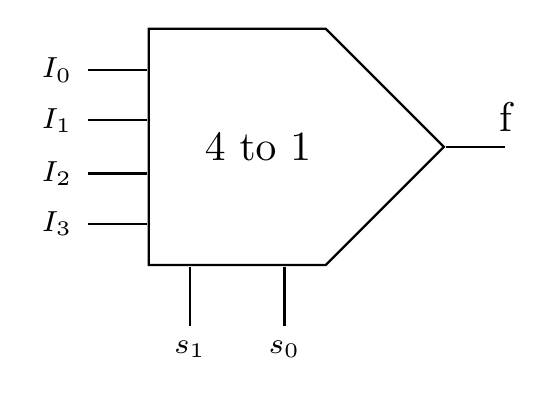
\begin{tikzpicture}[multiplexer/.style={
			draw,
			signal,
			shape border uses incircle, 
			shape border rotate=270,
			minimum width=2.5cm, 
			minimum height=2cm,
		}, thick,scale=1.5,every node/.style={transform shape}]
		\node[multiplexer] (mul) at (0,0) {~~~4 to 1};
		\draw (mul.east) --++(0.5cm,0) node[above]{f};
		
		\draw (mul.west)++(0, 0.65cm) --++(-0.5cm,0) node[left]{\scriptsize $I_0$};
		\draw (mul.west)++(0, 0.225cm) --++(-0.5cm,0) node[left]{\scriptsize $I_1$};
		\draw (mul.west)++(0, -0.225cm) --++(-0.5cm,0) node[left]{\scriptsize $I_2$};
		\draw (mul.west)++(0, -0.65cm) --++(-0.5cm,0) node[left]{\scriptsize $I_{3}$};
		
		\draw (mul.south)++(-0.4cm, 0) --++(0, -0.5cm) node[below]{\scriptsize $s_{1}$};
		\draw (mul.south)++(0.4cm, 0) --++(0, -0.5cm) node[below]{\scriptsize $s_{0}$};
	\end{tikzpicture}
\end{center}\bigbreak

If $s_1s_0 = (00)_2 \implies f=I_0$.\\
If $s_1s_0 = (01)_2 \implies f=I_1$.\\
If $s_1s_0 = (10)_2 \implies f=I_2$.\\
If $s_1s_0 = (11)_2 \implies f=I_3$.\\

The truth table (compact form) is\bigbreak

\begin{center}
	\begin{tabular}{|c|c||c|}
		$s_1$ & $s_1$ & $f$\\\hline
		  0   &   0   & $I_0$\\
		  0   &   1   & $I_1$\\
		  1   &   0   & $I_2$\\
		  1   &   1   & $I_3$\\
	\end{tabular}
	\bigbreak
\end{center}

Thus, the Boolean expression is $f = I_0\bar{s_1}\bar{s_0} + I_1\bar{s_1}s_0 + I_2s_1\bar{s_0} + I_3s_1s_0$. Now, we can draw the multiplexer circuit.\\

\begin{center}
	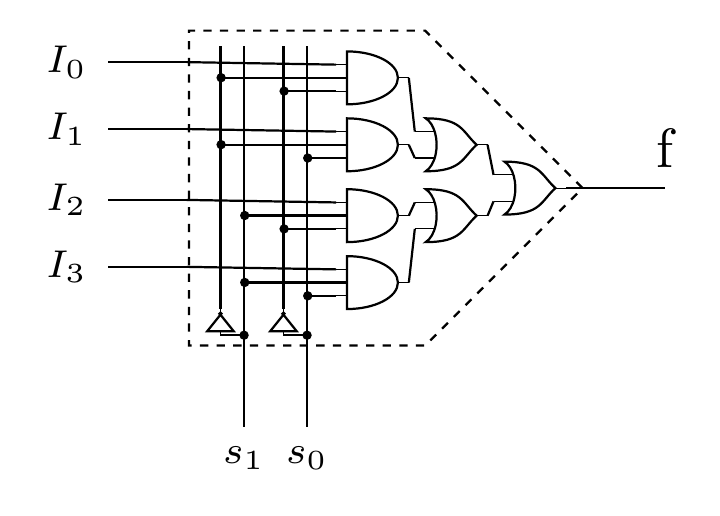
\begin{tikzpicture}[multiplexer/.style={
			draw,
			signal,
			shape border uses incircle, 
			shape border rotate=270,
			minimum width=2.5cm, 
			minimum height=2cm,
			dashed
		}, thick,scale=2,every node/.style={transform shape}]
		\node[multiplexer] (mul) at (0,0) {};
		\draw (mul.east) --++(0.5cm,0) node[above]{f};
		
		\draw (mul.west)++(0, 0.65cm)++(0, 0.15cm) --++(-0.5cm,0) node[left]{\scriptsize $I_0$};
		\draw (mul.west)++(0, 0.225cm)++(0, 0.15cm) --++(-0.5cm,0) node[left]{\scriptsize $I_1$};
		\draw (mul.west)++(0, -0.225cm)++(0, 0.15cm) --++(-0.5cm,0) node[left]{\scriptsize $I_2$};
		\draw (mul.west)++(0, -0.65cm)++(0, 0.15cm) --++(-0.5cm,0) node[left]{\scriptsize $I_{3}$};
		
		\draw (mul.south)++(-0.4cm, 0) --++(0, -0.5cm) node[below]{\scriptsize $s_{1}$};
		\draw (mul.south) --++(0, -0.5cm) node[below]{\scriptsize $s_{0}$};
		
		\draw (mul.south)++(-0.4cm, 0) -- (-0.4cm, 0.9cm);
		\draw (mul.south) -- (0, 0.9cm);
		
		\node at (-0.55cm, -0.85cm)[not port, rotate=90, scale=0.12, thin](Lnot){};
		\node at (-0.15cm, -0.85cm)[not port, rotate=90, scale=0.12, thin](Rnot){};
		\draw (Lnot.in) -- ++(0.15cm, 0) node[circle, fill, inner sep=0.6]{};
		\draw (Rnot.in) -- ++(0.15cm, 0) node[circle, fill, inner sep=0.6]{};
		\draw (Lnot.out) -- (-0.55cm, 0.9cm);
		\draw (Rnot.out) -- (-0.15cm, 0.9cm);
		
		\node at (0.6cm, 0.7cm)[and port, scale=0.3, thin](and0){};
		\node at (0.6cm, 0.275cm)[and port, scale=0.3, thin](and1){};
		\node at (0.6cm, -0.175cm)[and port, scale=0.3, thin](and2){};
		\node at (0.6cm, -0.6cm)[and port, scale=0.3, thin](and3){};
		\draw (mul.west)++(0, 0.65cm)++(0, 0.15cm) -- (and0.in 1);
		\draw (mul.west)++(0, 0.225cm)++(0, 0.15cm) -- (and1.in 1);
		\draw (mul.west)++(0, -0.225cm)++(0, 0.15cm) -- (and2.in 1);
		\draw (mul.west)++(0, -0.65cm)++(0, 0.15cm) -- (and3.in 1);
		
		\node at (1.1cm, 0.275cm)[or port, scale=0.3, thin](or1){};
		\node at (1.1cm, -0.175cm)[or port, scale=0.3, thin](or2){};
		\node at (1.6cm, 0)[or port, scale=0.3, thin](or3){};
		\draw (and0.out) -- (or1.in 1);
		\draw (and1.out) -- (or1.in 2);
		\draw (and2.out) -- (or2.in 1);
		\draw (and3.out) -- (or2.in 2);
		\draw (or1.out) -- (or3.in 1);
		\draw (or2.out) -- (or3.in 2);
		\draw (or3.out) -- (mul.east) --++(0.5cm,0);
		
		\draw (and0.in 2)++(0.07cm, 0.085cm)--++(-0.07cm, 0) --++(-0.18cm, 0)--++(-0.55cm, 0) node[circle, fill, inner sep=0.6]{};
		\draw (and0.in 2)--++(-0.18cm, 0)--++(-0.15cm, 0) node[circle, fill, inner sep=0.6]{};
		\draw (and1.in 2)++(0.07cm, 0.085cm)--++(-0.07cm, 0) --++(-0.18cm, 0)--++(-0.55cm, 0) node[circle, fill, inner sep=0.6]{};
		\draw (and1.in 2)--++(-0.18cm, 0) node[circle, fill, inner sep=0.6]{};
		\draw (and2.in 2)++(0.07cm, 0.085cm)--++(-0.07cm, 0) --++(-0.18cm, 0)--++(-0.4cm, 0) node[circle, fill, inner sep=0.6]{};
		\draw (and2.in 2)--++(-0.18cm, 0)--++(-0.15cm, 0) node[circle, fill, inner sep=0.6]{};
		\draw (and3.in 2)++(0.07cm, 0.085cm)--++(-0.07cm, 0) --++(-0.18cm, 0)--++(-0.4cm, 0) node[circle, fill, inner sep=0.6]{};
		\draw (and3.in 2)--++(-0.18cm, 0) node[circle, fill, inner sep=0.6]{};
	\end{tikzpicture}
\end{center}\bigbreak

\pagebreak
\subsubsection{The Decoder (2 to 4)}
\bigbreak

The decoder is the opposite of a multiplexer. Instead of encoding a larger input into a smaller output, it decodes a smaller input into a larger output. It is denoted with the following diagram.\\

\begin{center}
	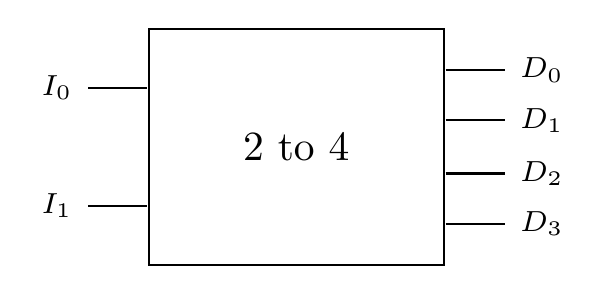
\begin{tikzpicture}[multiplexer/.style={
			draw,
			rectangle,
			shape border uses incircle, 
			shape border rotate=270,
			minimum width=2.5cm, 
			minimum height=2cm,
		}, thick,scale=1.5,every node/.style={transform shape}]
		\node[multiplexer] (mul) at (0,0) {2 to 4};
		
		\draw (mul.west)++(0, 0.5cm) --++(-0.5cm,0) node[left]{\scriptsize $I_0$};
		\draw (mul.west)++(0, -0.5cm) --++(-0.5cm,0) node[left]{\scriptsize $I_1$};
		
		\draw (mul.east)++(0, 0.65cm) --++(0.5cm,0) node[right]{\scriptsize $D_0$};
		\draw (mul.east)++(0, 0.225cm) --++(0.5cm,0) node[right]{\scriptsize $D_1$};
		\draw (mul.east)++(0, -0.225cm) --++(0.5cm,0) node[right]{\scriptsize $D_2$};
		\draw (mul.east)++(0, -0.65cm) --++(0.5cm,0) node[right]{\scriptsize $D_3$};
	\end{tikzpicture}
\end{center}\bigbreak

The truth table is

\begin{center}
	\begin{tabular}{|c|c||c|c|c|c|}
		$I_1$ & $I_0$ & $D_0$ & $D_1$ & $D_2$ & $D_3$ 	\\\hline
		  0   &   0   &   1   &   0   &   0   &   0  	\\
		  0   &   1   &   0   &   1   &   0   &   0  	\\
		  1   &   0   &   0   &   0   &   1   &   0  	\\
		  1   &   1   &   0   &   0   &   0   &   1  	\\
	\end{tabular}
	\bigbreak
\end{center}

The Boolean expressions are therefore:
\begin{center}
	$D_0 = \bar{I_1}\bar{I_0}$\\
	$D_1 = \bar{I_1}I_0$\\
	$D_2 = I_1\bar{I_0}$\\
	$D_3 = I_1I_0$
\end{center}

We can now draw the circuit diagram of the decoder:

\begin{center}
	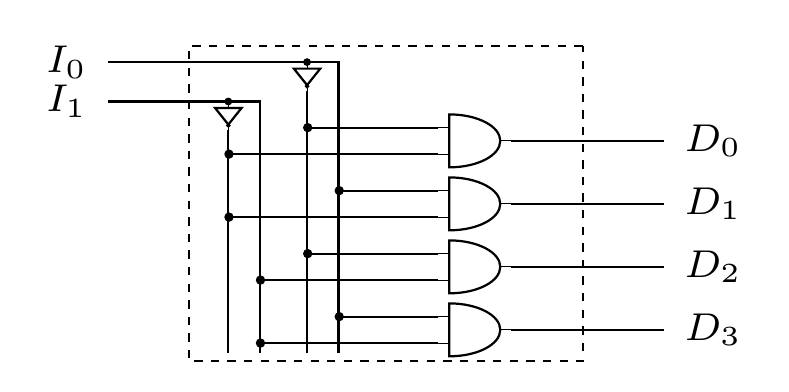
\begin{tikzpicture}[multiplexer/.style={
			draw,
			rectangle,
			shape border uses incircle, 
			shape border rotate=270,
			minimum width=2.5cm, 
			minimum height=2cm,
			dashed
		}, thick,scale=2,every node/.style={transform shape}]
		\node[multiplexer] (mul) at (0,0) {};
		
		\draw (mul.west)++(0, 0.9cm) --++(-0.5cm,0) node[left]{\scriptsize $I_0$};
		\draw (mul.west)++(0, 0.65cm) --++(-0.5cm,0) node[left]{\scriptsize $I_1$};
		
		\draw (mul.east)++(0, 0.4cm) --++(0.5cm,0) node[right]{\scriptsize $D_0$};
		\draw (mul.east)++(0, 0cm) --++(0.5cm,0) node[right]{\scriptsize $D_1$};
		\draw (mul.east)++(0, -0.4cm) --++(0.5cm,0) node[right]{\scriptsize $D_2$};
		\draw (mul.east)++(0, -0.8cm) --++(0.5cm,0) node[right]{\scriptsize $D_3$};
		
		\node at (0.75cm, 0.4cm)[and port, scale=0.3, thin](and0){};
		\node at (0.75cm, 0cm)[and port, scale=0.3, thin](and1){};
		\node at (0.75cm, -0.4cm)[and port, scale=0.3, thin](and2){};
		\node at (0.75cm, -0.8cm)[and port, scale=0.3, thin](and3){};
		\draw (mul.east)++(0, 0.4cm) -- (and0.out);
		\draw (mul.east)++(0, 0.0cm) -- (and1.out);
		\draw (mul.east)++(0, -0.4cm) -- (and2.out);
		\draw (mul.east)++(0, -0.8cm) -- (and3.out);
		
		\draw (mul.west)++(0, 0.9cm) -- (-0.30cm, 0.9cm) -- (-0.30cm, -0.95cm);	% i0
		\draw (mul.west)++(0, 0.65cm) -- (-0.80cm, 0.65cm) -- (-0.80cm, -0.95cm);	% i1
		\node at (-0.5cm, 0.8cm)[not port, rotate=-90, scale=0.12, thin](not0){};
		\node at (-1cm, 0.55cm)[not port, rotate=-90, scale=0.12, thin](not1){};
		\draw (not0.in) -- (-0.50cm, 0.9cm) node[circle, fill, inner sep=0.5]{};
		\draw (not1.in) -- (-1cm, 0.65cm) node[circle, fill, inner sep=0.5]{};
		\draw (not0.out) -- (-0.50cm, -0.95cm);
		\draw (not1.out) -- (-1cm, -0.95cm);
		
		\draw (and0.in 1)--++(-0.63cm, 0)--++(-0.2cm, 0) node[circle, fill, inner sep=0.6]{};
		\draw (and0.in 2)--++(-0.63cm, 0)--++(-0.2cm, 0)--++(-0.5cm, 0) node[circle, fill, inner sep=0.6]{};
		\draw (and1.in 1)--++(-0.63cm, 0) node[circle, fill, inner sep=0.6]{};
		\draw (and1.in 2)--++(-0.63cm, 0)--++(-0.2cm, 0)--++(-0.5cm, 0) node[circle, fill, inner sep=0.6]{};
		\draw (and2.in 1)--++(-0.63cm, 0)--++(-0.2cm, 0) node[circle, fill, inner sep=0.6]{};
		\draw (and2.in 2)--++(-0.63cm, 0)--++(-0.5cm, 0) node[circle, fill, inner sep=0.6]{};
		\draw (and3.in 1)--++(-0.63cm, 0) node[circle, fill, inner sep=0.6]{};
		\draw (and3.in 2)--++(-0.63cm, 0)--++(-0.5cm, 0) node[circle, fill, inner sep=0.6]{};
	\end{tikzpicture}
\end{center}\bigbreak

Note that we can only make $n$ to $2^n$ decoders: The number of outputs must always be a power of two.\\

For the 3 to 8 decoder, we would obtain the Boolean expressions: $D_0 = \bar{I_2}\bar{I_1}\bar{I_0}$, $D_1 = \bar{I_2}\bar{I_1}I_0$, ... $D_7 = I_2I_1I_0$.\\

\subsection{Memory Organization}
\bigbreak
\subsubsection{Computer Components}
\bigbreak

Modern computers are built using the \textbf{Von Neumann machine}. There are three aspects:

\begin{itemize}
	\item \textbf{Architecture}: \textbf{I/O} (User interaction) + \textbf{Memory} (Storage) + \textbf{CPU} (\textit{CPU}: Control Unit, \textit{ALU}: Arithmetic and Logic Unit). These are all connected by a shared bus.
	\item \textbf{Stored Programs}: All programs and data are stored in memory (binary).
	\item \textbf{Sequential Execution}: Also called the \textbf{fetch-decode-execute} cycle. Instructions are \textbf{fetched} from memory, \textbf{decoded} by the CPU and then \textbf{executed} by the ALU. If there is a result, it is stored back in memory. \smallskip
\end{itemize}

% Course Video 3
\subsubsection{Memory}
\bigbreak

The memory is organized in a \textbf{hierarchy}. At the bottom of the hierarchy is the Hard Drive (in TB). At the top is the CPU. Since the hard drive is slow, when some data from the hard drive is needed, it is first loaded into \textbf{RAM (Random Access Memory)} (in GB). The RAM is still too slow for the RAM, so the data is stored in \textbf{cache} (in KB or MB). Yet still, this is not fast enough for the CPU, so \textbf{registers} (in Bytes) in the CPU itself are used to store variables.

\begin{center}
	\tikzstyle{top} = [rectangle, minimum width=3cm, minimum height=1cm, text centered, draw=black, fill=purple!30]
	\tikzstyle{medtop} = [rectangle, minimum width=5cm, minimum height=1cm, text centered, draw=black, fill=red!30]
	\tikzstyle{medbot} = [rectangle, minimum width=8cm, minimum height=1cm, text centered, draw=black, fill=orange!30]
	\tikzstyle{bot} = [rectangle, minimum width=12cm, minimum height=1cm, text centered, draw=black, fill=yellow!30]
	
	\begin{tikzpicture}[node distance=2cm, >=latex', auto, thick]
		\node (ntop) [top] {CPU};
		\node (nmedtop) [medtop, below of=ntop] {Cache};
		\node (nmedbot) [medbot, below of=nmedtop] {RAM (Random Access Memory)};
		\node (nbot) [bot, below of=nmedbot] {Hard Drive};
		
		\path[->, shift left=2em]
		(ntop) edge node {store} (nmedtop)
		(nmedtop) edge node {load} (ntop);
		\path[->, shift left=3.5em]
		(nmedtop) edge node {update} (nmedbot)
		(nmedbot) edge node {load} (nmedtop);
		\path[->, shift left=6em]
		(nmedbot) edge node {save} (nbot)
		(nbot) edge node {load} (nmedbot);	
	\end{tikzpicture}
\end{center}
\bigbreak

\noindent As you \textbf{go up} the hierarchy, the \textbf{speed increases}, but the \textbf{size decreases} and the \textbf{cost increases}.

\subsubsection{RAM}
\bigbreak

Random access memory is organized in an array of Bytes ("words"). \\

Words in RAM are addressed with a byte themselves (e.g. 01101101 is an address). These are typically written in hexadecimal (e.g. 6D). \\

Words in RAM can be data or machine code instructions. Instructions contain a binary code for each operation (for example, addition). Instructions codes are dependent on the CPU.\\

For an $n$-bit computer system, there are $2^n$ bytes in memory (addressed in decimal with 0 to $2^n-1$). \\

The size of the RAM is equal to the number of cells in memory times 1 byte. Thus, \textit{the max size of the RAM in a $n$-bit computer is $2^n$ bytes}. For example, in a 32-bit computer, the (max) size of the RAM is $2^{32}$ bytes. This is a large number that is hard to get a grasp of, so we will use prefixes to denote larger numbers of bytes.\\

Namely, a \textbf{kilobyte} (KB) is $2^{10} = 1024 \approx 1000$. A \textbf{megabyte} (MB) is $2^{20}$, a \textbf{gigabyte} (GB) is $2^{30}$, a \textbf{terabyte} (TB) is $2^{40}$, and so on.\\

We can write $2^{32}\text{ bytes} = 2^{2} \times 2^{30}\text{ bytes} =$ 4 GB. Thus, the max memory size of a 32-bit computer is 4 GB.\\

If instead we had a 64-bit computer, the max RAM size is $2^{64}\text{ bytes} = 2^{24} \times 2^{40}\text{ bytes} = 2^{24}$ TB. This is a very large number and totally impractical in real life. Therefore, in a 64-bit computer, we do not need to display memory addresses with the full 64-bits. The data it is necessary to, but not the memory addresses.\\

It is important to always distinguish between the address and content of a cell in memory. For example, the content could store the value 15, but the address is 34. \\


\subsubsection{Memory Basic Operations}
\bigbreak

There are 2 basic operations. \\

Firstly, the \textbf{fetch} operation: Reads data from the memory. The idea is that we want to get a value from memory using a fetch operation, but we need to know where to get this value, so we use an \textit{address} (value = fetch(address)). For example, value = fetch(34) returns the value 15 (which is stored in the memory address 34).\\

Secondly, the \textbf{store} operation: Stores data into memory. We need both a value and an address (store(value, address)) For example, stores(22, 34) would store the value of 22 in adress 34.\\

How can we do this in hardware?\\

To do this, we will discuss \textbf{registers}. Registers are storage cells (capacity in bits) and is located outside of the RAM (for example, in the CPU). \\

A system is equipped with 2 registers: \\
The \textbf{MDR:} Memory Data Register. It contains data read from (or to be stored in) memory. \\
The \textbf{MAR:} Memory Address Register. It contains the address for fetch \textit{or} store. \\

For example, the MAR allows us to select a location in memory and the MDR allows us to transfer data from or to memory.\\

In a \textit{fetch} operation, the steps are as follows:

\begin{itemize}
	\item Put address in MAR
	\item Read
	\item Data is sent to MDR
\end{itemize}

In a \textit{store} operation, the steps are as follows:

\begin{itemize}
	\item Put address in MAR
	\item Put data in MDR
	\item Write
\end{itemize}


\subsubsection{Address Decoding}
\bigbreak

The MAR will have $N$ bits of memory. How to we select a location in RAM given a certain address in the MAR? We need a circuit that takes in $N$ bits and gives $2^N$ outputs (one for each address in memory). Thus, the circuit that does this is a \textbf{$\mathbf{N}$ to $\mathbf{2^N}$ bit decoder}. This is called \textit{address decoding}.\\


\subsubsection{Arithmetic and Logic Unit}
\bigbreak

The CPU is composed of the ALU and the CU.\\

The Arithmetic and Logic Unit (\textbf{ALU}) is responsible for implementing arithmetic and logic operations (A+B, A-B, A==B). \\

The ALU contains

\begin{itemize}
	\item Registers to store operands and result
	\item Combinational circuits for operations (+, -, *, ==)
	\item Selection circuit (for operation)
\end{itemize}

Let us assume that we have 16 registers: $R_0$, $R_1$, ..., $R_0$.\\

We select a register for the left operand (eg. A), another register for the right operand (B), and a last for the operation (+).\\

In summary, there is a selection circuit to select the left and right operands (this is performed by the CU). The result of this selection is connected to all the operations (+/-, <, ==, etc.), but only one operation is of interest. The desired operation output is selected by a multiplexer which returns the value to a register. The selection lines come from the CU.\\

\subsubsection{Control Unit}
\bigbreak

The control unit (\textbf{CU}) is responsible for the ALU operations and memory operations, but most importantly is responsible for executing the stored program.\\

The CU will fetch (memory operation), decode (select operation in ALU) and execute (select in ALU and save to memory).\\

The stored program is binary, but written in \textbf{machine language} instructions. \\

Machine language is not C++ or Java or Python. These are high level languages (designed for programmers). Machine language is a low level language (designed for the computer).\\

To go from a high level language to a low level language, we use a \textbf{compiler}. For example, the compiler translates C++ to machine language (binary).\\

Machine language varies across CPU architecture (or brand, such as Intel or AMD) uses its own set of machine instructions. For example, 64-bit AMD CPUs uses the AMD64 instruction set and Intel uses the X86 or X64 instruction set.\\

We can divide machine instructions into 

\begin{itemize}
	\item Data transfer
	\item Arithmetic
	\item Compare
	\item Branch
\end{itemize}\bigbreak


\subsection{Machine Language Instructions}
\bigbreak

We will define a simple machine language for pedagogical reasons. 

\subsubsection{Data Transfer}
\bigbreak

Data transfer instruction moves data between the CPU and memory. We will define the following 3 instructions:\\

\textbf{LOAD X}: Loads a register R in the CPU with the content of memory at address X. We write: Con(R) = Con(X). Con stands for content.\\

\textbf{STORE X}: Stores the content of R in memory at the address X.\\

\textbf{MOVE X, Y}: Copies the content at memory address X into the memory address Y. We write: Con(Y) = Con(X).\\


\subsubsection{Arithmetic}
\bigbreak

There are many possible arithmetic operations, but we will define the following instructions as an example:\\

\textbf{ADD X, Y}: Con(X) = Con(X) + Con(Y).\\
\textbf{ADD X}: Con(R) = Con(X) + Con(R). R is a predetermined register (which you must load a value into prior, and store a value from after).\\

There are many more.\\

\subsubsection{Compare}
\bigbreak

To implement the compare operation, the CPU performs a subtraction and based on the sign (+ or -) and magnitude of the result (0 or not) returns a value.\\

The CPU sets the values of the \textbf{Condition Code Register} (CCR). There are three bits in the CCR. The less than (LT), the equal (EQ), and the greater than (GT):

\[
\renewcommand\arraystretch{1.5}
\begin{array}{C|C|C|C|}\cline{2-4}
	CCR: & LT & EQ & GT \\\cline{2-4}
\end{array}
\]\bigbreak

We define the following instruction:

\begin{equation*}
	\text{\textbf{COMPARE X, Y}: }\begin{cases}
		\text{GT=1, EQ=0, LT=0} \quad &\text{if} \, \text{Con(X) > Con(Y)} \\
		\text{GT=0, EQ=1, LT=0} \quad &\text{if} \, \text{Con(X) = Con(Y)} \\
		\text{GT=0, EQ=0, LT=1} \quad &\text{if} \, \text{Con(X) < Con(Y)} \\
	\end{cases}
\end{equation*}\bigbreak


\subsubsection{Branch}
\bigbreak

In the memory, we have the program memory which are the set of instructions that the computer uses to run. \\

To go to a different part in the program (jump across instruction lines in memory), we need to use a branch instruction. This allows to jump to an instruction stored at a specified address in memory. \\

\textbf{JUMP X}: The next instruction to execute is stored at the memory address X.\\

\textbf{JUMPGT X}: Jump to X only if GT = 1 (otherwise, no effect). \\
\textbf{JUMPEQ X}: Jump to X only if EQ = 1.\\
\textbf{JUMPLT X}: Jump to X only if LT = 1.\\
These instruction must be proceeded by a compare operation.\\

\textbf{HALT}: Stops the program.\\

\subsubsection{Example: Arithmetic Operation}
\bigbreak

If we want to perform the psudeocode:\\

Set a = b + c + d\\

then we would have the following in program memory: \\

\begin{center}
	\begin{tabular}{c|l|}\cline{2-2}
		50 & LOAD 101 \\\cline{2-2}
		51 & ADD 102 \\\cline{2-2}
		52 & ADD 103 \\\cline{2-2}
		53 & HALT \\\cline{2-2}
		... & ... \\\cline{2-2}
		100 & a \\\cline{2-2}
		101 & b \\\cline{2-2}
		102 & c \\\cline{2-2}
		103 & d \\\cline{2-2}
		... & ... \\\cline{2-2}
	\end{tabular}
	\bigbreak
\end{center}

What occurs is that first a is loaded into R, then b is added to the content of R, then d is added to the content of R. Finally the program is halted.\\

\subsubsection{Example: Conditional}
\bigbreak

If we want to perform the psudeocode:\\

\setlength{\parindent}{0.5cm}\noindent
If (a == b) then\\
\indent Set c = d\\
Else\\
\indent Set c = b\\
Stop\\
\setlength{\parindent}{0pt}

then we would have the following in program memory: \\

\begin{center}
	\begin{tabular}{c|l|}\cline{2-2}
		50 & COMPARE 100, 101 \\\cline{2-2}
		51 & JUMPEQ 54 \\\cline{2-2}
		52 & MOVE 101, 102 \\\cline{2-2}
		53 & JUMP 55 \\\cline{2-2}
		54 & MOVE 102, 103 \\\cline{2-2}
		55 & HALT \\\cline{2-2}
		... & ... \\\cline{2-2}
		100 & a \\\cline{2-2}
		101 & b \\\cline{2-2}
		102 & c \\\cline{2-2}
		103 & d \\\cline{2-2}
		... & ... \\\cline{2-2}
	\end{tabular}
	\bigbreak
\end{center}

First, we compare the content at address 100 (a) to the content at address 101 (b). Then, we conditionally jump if EQ = 1, set c = d and then halt. Otherwise, we continue on and set c = b before jumping to the halt.\\

\subsubsection{Example: Loop}
\bigbreak

If we want to perform the psudeocode:\\

\setlength{\parindent}{0.5cm}\noindent
While (a < b) then\\
\indent Set a = a+c\\
EndWhile\\
Stop\\
\setlength{\parindent}{0pt}

then we would have the following in program memory: \\

\begin{center}
	\begin{tabular}{c|l|}\cline{2-2}
		50 & COMPARE 100, 101 \\\cline{2-2}
		51 & JUMPEQ 57 \\\cline{2-2}
		52 & JUMPGT 57  \\\cline{2-2}
		53 & LOAD 100 \\\cline{2-2}
		54 & ADD 102 \\\cline{2-2}
		55 & STORE 100 \\\cline{2-2}
		56 & JUMP 50 \\\cline{2-2}
		57 & HALT \\\cline{2-2}
		... & ... \\\cline{2-2}
		100 & a \\\cline{2-2}
		101 & b \\\cline{2-2}
		102 & c \\\cline{2-2}
		... & ... \\\cline{2-2}
	\end{tabular}
	\bigbreak
\end{center}

First, we compare a to b. Then, we conditionally jump to the halt if EQ = 1 or if GT = 1. If not, we load a in R, add c, store the content of R back into a, and then jump back up to the compare. \\





\end{document}
